\section{Discussion}
\label{sec:discussion}

\subsection{Overview of key findings}

The $N = 1426$ data support a six-factor architecture at three levels of distinction, none reducible to the others. The first level is content constructs of the psyche: internal dissonance (ID) as a signature of blocking defensive work, childhood alienation (CA) as environmental history, psychopathy (P) as the moral signature ``this is permitted to me'', affective and cognitive empathy (\EAF{}, \Ecog{}) as two distinguishable functions, masking (M) as a regulatory layer. The second level is their structural geometry: ID and P are statistically separable and describe two different channels of empathy loss (passive blocking and active narrative); \Ecog{} and \EAF{} are non-equivalent and dissociate under different conditions; M is a weak, poorly differentiated factor ($\omega = 0.546$) not ready to sustain independent conclusions. The third level is attention (A) as a structurally distinct element: not content of the psyche but condition of its organization. A moderates both segments of the CA$\to$ID$\to$\EAF{} channel in the narrow specification and transforms the classical picture of traumatic damage into the profile of an integrated survivor. These results reproduce what has been described across disparate literatures but not yet woven into a single psychometric fabric.

\paragraph{The central empirical shift: what breaks empathy is defense, not trauma.} Before moving to the reading of factors, we lift one result that reformulates a century-old clinical intuition. In the baseline regression CA predicts \EAF{} negatively (total effect $c = -0.129$, 95\% CI $[-0.184, -0.073]$) --- the sign consistent with the standard picture ``trauma suppresses empathy''. But once ID is included as a mediator, the direct effect of CA on \EAF{} \emph{changes sign} to positive ($c' = +0.073$, 95\% CI $[+0.018, +0.128]$). Put differently: if the defensive structure that trauma built is not accounted for, the association between childhood history and reduced adult empathy is visible; if the defensive structure is accounted for, childhood history in itself is weakly positively associated with affective empathy, and the negative effect passes entirely through the ID channel. This is not a statistical artifact and not cosmetic --- it shifts the causal point of therapeutic application: the work is not with the past as such, but with the defense built between past and present. The clinical intuition, present since \citet{freud1917}, that ``trauma requires working-through'' receives an operational refinement --- what needs to be worked through is not the event, but the defensive structure the event left behind. This is also the basis for §\ref{subsec:integrated_survivor} on the integrated survivor: once the defensive structure is metabolized, the \emph{positive} component of the CA $\to$ \EAF{} link becomes observable at group level, not merely a hidden statistical residual.

We do not offer a new theory of empathy. We offer a \emph{measurement scaffolding} in which constructs already described in different traditions acquire shared coordinates and testable mutual relations. This does not mean the model is metaphysically neutral --- every measurement carries an ontological commitment about what it measures. We do not hide this behind the rhetoric of ``we are just psychometricians''. We assert directly: the six \DEIC{} functions correspond to real structure in a weak but concrete sense --- this structure generates predictions that may fail, and if they fail in pre-registered replication, the model is refuted at the corresponding point. What we do not claim is a ready-made theory of the psyche as a whole; what we do claim is that what was measured correlates with what is there.

\subsection{Three points of empirical resistance to the frame}
\label{subsec:data_resistance_en}

A worldview-first project (see §\ref{subsec:worldview_first}) is legitimate only to the extent that the data resist the original frame in concrete, central places. We gather those places explicitly here, because in the results sections they are scattered and their cumulative weight is easy to lose.

\paragraph{First --- the collapse of \IMM{} in the unified SEM.} In the narrow specification of the CA$\to$ID$\to$\EAF{} channel with A as a double moderator of both stages, $\IMM = -0.00197$ with a significant bootstrap CI. This was one of the central anticipated confirmations: A was expected to restructure the whole channel. In the unified SEM --- where P, A, M are included simultaneously as parallel mediators and main effects --- \IMM{} collapses to $+0.0001$ (NS). This is not an artifact: it is re-composition of variance. The main explanatory weight on \EAF{} at the population level is carried not by the ID$\times$A product but by P as direct negative predictor ($b = -0.726$) and A as direct positive predictor ($b = +0.393$). We were forced to reformulate: the ID-A modulation remains substantively meaningful at the level of individual trajectory (§\ref{subsec:architecture}), but at the population level the principal variance in affective empathy concentrates in the P narrative and the A presence. This is a weaker claim than the one we started with.

\paragraph{Second --- SUP refuses to be part of passive blocking.} In the original frame, the five wave-1 defensive subscales were expected to assemble into a single ID latent as distinct surfaces of one containing system. The bifactor analysis showed: per-subscale ECV for SUP $= 0.31$ (69\% of SUP variance is unique and not explained by general ID), composite correlations SUP $\leftrightarrow$ IDS $= 0.05$ and SUP $\leftrightarrow$ DIS $= 0.11$. Phenomenologically this falls into place: suppression is an ego-syntonic conscious action in which the subject \emph{chooses} not to feel, and it sits structurally closer to the P architecture of conditional access than to dissociation, isolation, flattening as automatic ego-dystonic mechanisms. In the pre-data frame, SUP and DIS were treated as isomorphic indicators of one system; after the data, SUP must be carried as a separate latent in wave 2. This is not an adjustment inside the frame; it is a change in the topology of defenses.

\paragraph{Third --- A refuses to be a latent.} We expected witnessing to behave as an ordinary reflective latent: a set of items loading on a common attention factor. A-CFA Tier 5 with a carefully curated set of 17 items yields CFI $= 0.87$, RMSEA $= 0.08$, and --- more importantly conceptually --- a signature \emph{sign reversal} of \IMM{} when the latent A is substituted for the composite. Sign reversal on purification is a diagnostic hallmark of a formative rather than reflective structure: A has no common variance core that can be extracted from items, because A is not an internal trait manifesting in behavior but a field-condition, a \emph{mode} in which other functions exist (§\ref{subsec:A_as_field_condition}). This is the most substantial of the three revisions: it reclassifies the central moderator of the program from an ordinary psychometric construct into an ontologically distinct type of object. Wave 2 requires a dedicated A-scale, constructed formatively by design, with explicit methodological work on the consequences.

These three points are not a routine list of limitations. They are the places where the data genuinely forced the frame to bend: an expected effect disappeared, an expected structure dissolved, an expected construct type turned out to be different. The presence of these three shifts is the primary evidence available to us that the frame is not self-confirming. Had the data not resisted anywhere, the work would merit being read as decorative empiricism. They resisted, and the resistance is named.

\subsection{What the three new validation analyses give together}
\label{subsec:validity_package}

The three subsections §\ref{subsec:free_text_convergent}, \ref{subsec:roc_validity}, and \ref{subsec:dx_count_bias} address the same question from three independent angles: to what extent do DEIC constructs measure what they are named, and what exactly do they measure in comparison with standard clinical proxies. We bring these three results into the discussion as a single package, because taken individually they read as technical validation reports, but taken together they become a structural claim.

\emph{Convergently}, the P scale is supported by direct free-text self-description (manipulation\_callousness $N = 10$, $d_P = +2.32$, AUC $= 0.964$), with P retaining significance in a multivariable model with the full set of covariates. \emph{Architecturally}, the separation of the P and ID channels is reproduced on behavioral anchors: manipulation\_callousness activates P without D; social\_isolation activates D without P. These two poles are empirical ``crystalline examples'' of the two contours the model describes. \emph{Discriminantly}, P shows systematically lowered ROC ($\mathrm{AUC} \leq 0.42$) across all eight self-reported diagnostic categories: a construct measuring the architecture of conditional access and the moral narrative ``it is allowed for me'' should, by definition, not predict seeking a diagnosis; it predicts its \emph{absence}, and this is empirically confirmed. Symmetrically, CA shows $\mathrm{AUC} = 0.69$--$0.76$ for three early-trauma clusters (trauma, self-harm, personality); A yields $\mathrm{AUC} \leq 0.46$ for most clusters as a resource-predictor of the absence of clinical decompensation.

The three signatures are coherent. They mean: \DEIC{} does not replace DSM and is not reducible to it. DEIC measures an axis structurally \emph{orthogonal} to the logic of self-report clinical diagnosis: P respondents are architecturally invisible to dx-centered instruments, CA respondents are architecturally visible through an early-trauma signature, A respondents are architecturally protected from decompensation. This is the empirical justification for using DEIC \emph{alongside} standard diagnostics in the clinic, rather than in place of them or as an upstream proxy. DEIC captures what self-report DSM does not; self-report DSM captures what DEIC specifically does \emph{not} capture.

The second implication is methodological. $\texttt{dx\_count}$ as a severity measure in a DEIC-population is architecturally rather than merely statistically biased: it rises monotonically along the early-trauma axis but falls with the active P profile, so it builds into itself the very asymmetry of visibility that the P construct describes. In this paper we use $\texttt{dx\_count}$ only for descriptive characterization of the sample; formal clinical validation requires a wave with structured diagnosis (§\ref{subsec:wave2_design}).

\subsection{The architecture of six factors --- a brief reading}

\textbf{ID (internal dissonance)} is not a ``symptom'' but a signature that regulation is active and operating in blocking mode. High ID means that a conflict is present inside the psyche, and some of the affective content signals its own suppression. In psychoanalytic terms, this is what \citet{ferenczi1933} and \citet{klein1946} described as splitting and cleaving; in attachment terms, disorganized internal working models \citep{main1986}. Our contribution is a psychometric coordinate that can be measured, reproduced, and related to outcomes.

\textbf{CA (childhood alienation)} is a narrow environmental antecedent, not the full ACE syndrome. It is precisely the \emph{experience of mismatch} in the family of the earliest years: when the child's inner states do not meet an adequate response, and the family field becomes structurally incompatible with its own emotional experience. In our data CA predicts ID and distancing more strongly than the general ACE index. This aligns with mentalization theory \citep{fonagy2002}: not trauma as such, but the absence of a mentalizing response, forms the predisposition.

\textbf{P (psychopathy)} is the moral narrative ``this is permitted to me''. In \DEIC{} this construct is \emph{separate} from the architecture of affective coupling (see §\ref{subsec:architecture}): P is a layer of permission, not a layer of capacity. Partial $r$(P, \Ecog{}) after partialling ID and CA $= +0.32$ --- that is, in people with high P cognitive empathy is, if anything, \emph{elevated} rather than diminished. This is consistent with what \citet{blair1995, blair2013} and \citet{baroncohen2011} described: the psychopathic pattern includes a narrative layer of self-justification as an independent construct, not derivative of the affective level. In our formulation --- ``the capacity to understand others without feeling the moral obligation'' --- this is not a description of a broken function but a description of a specific combination of architecture (conditional coupling) and narrative (permission). \citet{cleckley1941} is the first literary description of this structure.

\textbf{\EAF{} / \Ecog{}} are partially confounded in the original instrument; the post-hoc factor separation resolved the paradox $r_{\mathrm{latent}}(P, E) = +0.35$ in the original model. Wave-2 scales must separate these two constructs by design. \citet{shamaytsoory2011} in the neuropsychological literature defends this dissociation; our psychometrics independently reproduces it.

\textbf{M (masking)} is a regulatory layer between the internal state and its external presentation. In the current instrument M is weakly instrumented and imprecisely differentiated from P ($r_{\mathrm{latent}} = +0.82$); reliability $\omega = 0.546$ does not permit M-specific conclusions. We keep M in the model as a placeholder for a future scale but do not rest any claims on it in this paper.

\textbf{A (attention)} is set out separately in the following section because it has a special ontological status.

The key geometry between these factors is as follows: P and ID are orthogonal (different mechanisms of empathy loss); \EAF{} and \Ecog{} are separable (different functions of empathy); CA precedes ID in temporal causality (age-stratified mediations are stable); and A moderates both stages of the CA$\to$ID$\to$\EAF{} channel in the narrow specification.

\subsection{A as condition of the field, not content of the field}
\label{subsec:A_as_field_condition}

The deepest theoretical distinction in the \DEIC{} architecture is not \emph{which} factors enter the model, but the fact that \emph{they do not all share the same ontological status}. ID, CA, P, M, \EAF{}, \Ecog{} are content factors, answering the question ``what is present in this person's psyche''. Attention (A) is a structurally different factor, answering a different question: ``is there inside this psyche a witnessing relation as such''. This distinction is not lexical.

The empirical trace of this distinction is three independent results. First, the attempt to construct a higher-order ``Integration'' factor over \{A, $-$M, \EAF{}, $-$ID\} yields catastrophically poor fit (CFI $= 0.71$, RMSEA $= 0.55$), and the correlation of the resulting INT\_score with A equals $0.995$. This means that ``integration'' as a separate construct above A does not exist --- A \emph{is} integration as measured by our composite procedure. Second, the conditional-process SEM with the A-composite as moderator shows that A is not simply added as a predictor but \emph{restructures} the CA$\to$ID$\to$\EAF{} channel. The Index of Moderated-Moderated Mediation $\IMM = -0.00197$, 95\% CI $[-0.00533, -0.00005]$ --- significant in the narrow specification, and at high values of A the canonical damage path changes sign. Third, and most strongly, the Tier-5 A-CFA on a carefully selected 17-item metacognitive pool yields acceptable fit (CFI $= 0.866$, RMSEA $= 0.081$) and high reliability ($\omega$ by absolute loadings $= 0.947$), but reveals a \emph{bipolar} factor structure: 8 items load one way, 9 in the opposite direction, despite a priori polarity alignment. When this latent A is substituted into the same conditional-process SEM in place of the theoretically weighted composite, the signs of the main coefficients flip (A $\to$ ID moves from $-0.626$ to $+0.659$), and \IMM{} loses significance.

We chose not to hide this result but to make it the centre of this section. It means the following: in the current pool of metacognitively phrased items ``I notice my internal states'' two different constructs are conflated. One is \emph{witnessing} proper, observation-of-observation, a testimonial relation that functionally weakens the ID$\leftrightarrow$\EAF{}-suppression coupling. The other is \emph{trauma hypervigilance}, a painful hyper-alertness to internal states, which correlates with ID positively and characterizes precisely the traumatized state, not the integrated one. A naked CFA does not distinguish them; a theoretically weighted composite into which this distinction is built in advance does.

From this follows a methodological conclusion that we treat as \emph{empirical grounds} for our position, not a caveat: A in the current instrument is a formative, not a reflective, construct. The main result (\IMM{} via A-moderation) was obtained under theoretically correct weighting; the robustness check on the bare latent A shows that witnessing as a separate construct needs to be reinstrumented, with items that explicitly distinguish observation-of-observation from internal hypervigilance. This is the first-priority task for wave~2.

That witnessing is a structurally different layer, not another content of the psyche, is a claim that various lines of thought have made independently over at least two and a half millennia. We do not bypass this literature or turn it into decorative backdrop; we work directly within its corpus. In advaita-vedanta this is \textit{sākṣī}, the witness --- the layer in which all other states are observed and which itself is not a state \citep[via][]{godman1985, nisargadatta1973}. In dzogchen it is \textit{rigpa}, primordial awareness, distinguished from \textit{sems} (ordinary mind-content) as a structurally different mode of consciousness. In Buddhist \textit{satipaṭṭhāna} tradition it is mindfulness in its original, non-reduced-to-behavioral-skill form: recollection of presence, not a concentration technique. In Gurdjieff --- ``self-remembering'' \citep[via][]{ouspensky1949}, the direct demand to hold the witnessing relation simultaneously with the observed action; in Fourth Way texts this function is set apart from emotional and cognitive functions as structurally autonomous. In psychoanalysis the same asymmetry appears in the ``observing ego'' \citep{sterba1934, kris1956} and takes modern form in mentalization in \citet{fonagy2002}. In cognitive science of the last two decades --- meta-awareness as a separate capacity described by \citet{dunne2011} on a Buddhist-philosophical basis, \citet{josipovic2014} in the non-dual frame, \citet{grabovac2011} in their Buddhist Psychological Model. \citet{lutz2008} show directly that contemporary clinical mindfulness science has inherited only one of several distinguishable functions of the original construction.

We name these lines not as ``allusions'' and not as ``parallel descriptions'' that \DEIC{} supposedly assembles into a single map. We name them because each of them within its own system works with the same structural distinction that emerges empirically in our data --- the bipolar latent structure on the metacognitive items, whose signature is compatible precisely with the hypothesis that witnessing and trauma hypervigilance are two different constructs beneath a single linguistic surface. When these traditions distinguish witnessing from the inner activity of consciousness, they distinguish the same thing we are now uncovering in the latent geometry. The epistemological order, accordingly, is the reverse of the one in which ``integrative'' projects usually place traditions: it is not they that are embedded in our model, but our coordinate that tests whether we have managed to catch the distinction they have been holding for millennia without statistical apparatus. The Bayesian prior on divergence is ``we have not yet measured what they distinguish'', not ``they were wrong''.

This leads directly to the difference between A and mindfulness as operationalized in FFMQ or in MBSR protocols. FFMQ measures dispositional behavioral characteristics of attention and non-judgment --- the observable level, amenable to skill training. Our A (in its correct formative form) is oriented to the \emph{presence of the witnessing relation as such}, which is structurally distinct from any observable behavioral characteristic. This is not a methodological quibble: \citet{vandam2018} in ``Mind the Hype'' document that the contemporary clinical mindfulness industry systematically flattens the living contemplative function to behavioral skill training, and that the psychometric toolkit developed inside this industry inherited the flattening as a structural feature. Our work at this point does not politely diverge from the MBSR literature but points directly: what \textit{satipaṭṭhāna} means, what advaita calls \textit{sākṣī}, dzogchen calls \textit{rigpa}, and Gurdjieff calls ``self-remembering'' --- is covered by none of the existing mindfulness scales. Psychometrics must return to this layer rather than settle for what is convenient to measure.

\subsection{The integrated survivor: compensation, not invulnerability}
\label{subsec:integrated_survivor}

One of the most important consequences of A-moderation of the CA$\to$ID$\to$\EAF{} channel is the existence of a subgroup of \emph{integrated survivors}. In our data this is $n = 118$ of 710 (17\%), for whom \emph{both} CA (childhood alienation above the median) and A (attention above the median) are high. This subgroup has the \emph{highest} \EAF{} values in the sample ($+0.37$), higher than people without trauma, for whom \EAF{} $= 0$ by construction. Interpretation: integrated trauma is a resource of empathy, not merely its obstacle.

This is not a romanticization of trauma or a denial of its damage. The baseline CA$\to$ID$\to$\EAF{} channel in the sample as a whole is negative and reproduces robustly; most people with high CA have reduced \EAF{}. The compensation effect works specifically in those who over the course of their life have developed the capacity to hold a witnessing relation to their own states (often, but not always, after therapy or contemplative practice). This is an empirically testable claim, not a normative one.

The substantive mechanism of compensation follows directly from the symmetric nature of the channel CA originally damaged. If ID is a general blocking of the containing function --- the inability to hold affect in both directions at once --- then A works through that same general channel: by developing witnessing toward one's \emph{own} states, the person develops the very containing capacity that had failed to form earlier. As a result, the capacity to sustain affective resonance with another is restored as well. We understand others better precisely to the extent that we can sustain our own internal material, and vice versa. Clinically, this is expressed in \citet{fonagy2002} as the principle of mentalization-based therapy: the goal is not to ``raise empathy toward others'' but to restore reflective function, which is by definition bidirectional; when it is restored, empathy toward others returns as a consequence, not as an independently trainable capacity. This is precisely why the path through A yields \EAF{} \emph{above} baseline: a person who has moved through the structural absence of a mentalizing field and has assembled it by their own work has their containing function structurally exposed, known from the inside, and therefore more sensitive than in someone for whom it has always operated unconsciously. This is not a metaphor but a mechanism: one's own knowledge of what precisely a blocked psyche fails to hold makes resonance with another blocked psyche more accurate.

Clinically, this reformulates the goal of trauma therapy: not to eliminate ID or CA (which is impossible and unnecessary), but to raise A to a point where ID ceases automatically to block \EAF{}. This aligns with what practices with a high share of somatic and witnessing work (somatic experiencing \citep{levine2015}, IFS \citep{schwartz1995}, sensorimotor psychotherapy \citep{ogden2006}, and a range of psychodynamic approaches with emphasis on mentalization \citep{fonagy2008}) show in clinical studies. It diverges from attempts to work on the cognitive level only --- we return to this in §\ref{subsec:relation_to_theories}.

For the public layer this result carries particular weight. ``Trauma is not a verdict'' is what people with childhood alienation want to hear, and in our research this is empirically defended. But the form of the message requires caution: fragmented trauma without A is not compensated; A-work is long and not always accessible; the CA$\times$A results should be communicated as a direction of work, not as a moral or motivational demand placed on the injured.

\paragraph{Two trajectories in hi-A: constitutional and integrated-traumatic.} It is important to separate the integrated-survivor profile explicitly from the general set of people with high A, because at the level of narrative the two easily merge. In our data hi-A (above the median) is distributed between two trajectories with a clear quantitative imbalance in favor of the first. In the $2\times 2$ classification, hi-CA $\cap$ hi-A gives $n = 118$, whereas lo-CA $\cap$ hi-A gives $n = 189$; that is, among hi-A, 62\,\% are non-traumatized people with a developed witnessing stance, and only 38\,\% are integrated-survivors. Tightening the ``healthy'' criterion (top 20\,\% on A, $N = 294$) shows that 75.9\,\% of them have no self-reported diagnosis, 51\,\% have simultaneously low (below median) CA, ACE, and ID, and 8\,\% meet the strict criterion of ``low on \emph{all} defensive composites'' (masking, lie, dissociation, flattening). Within hi-A, the internal correlations remain: $r$(A, CA) $= -0.28$, $r$(A, ID) $= -0.36$, $r$(A, dissociation) $= -0.53$, $r$(A, \EAF{}) $= +0.43$---the higher A within hi-A, the cleaner the profile. This means that at the population scale hi-A is predominantly represented not by ``former trauma survivors who have moved through integration,'' but by people with \emph{constitutionally} low defenses and without clinical history. The integrated survivor remains a structurally important subgroup---its existence anchors the thesis ``trauma is not a verdict'' and reformulates the goal of trauma therapy (A-work rather than the elimination of CA)---but it is a quantitative minority within hi-A, not a description of hi-A as such. Public communication of this result must hold this two-component structure: A is not a diagnostic marker of ``a person who has worked through trauma,'' but a field-condition that in our sample is more often registered in people without a history of trauma.

\subsection{Path A and path B: integration versus spiritual bypass}
\label{subsec:bypass}

The integrated survivor (§\ref{subsec:integrated_survivor}) is one of two possible trajectories that look similar on the surface in the coordinates of \DEIC{} but have opposite architectural structure and opposite clinical outcomes. Let us call them \textbf{path A} and \textbf{path B}. Along both, a rise of witnessing is registered in cross-sectional data. The difference lies in what happens to the ID channel simultaneously.

On path A---\emph{genuine integration}---the rise of A is accompanied by active work on the defensive structure: ID does not disappear (which is neither possible nor necessary), but it ceases to block \EAF{} automatically, becomes conscious, is metabolized. Phenomenologically this is the clinic of somatic experiencing \citep{levine2015}, IFS \citep{schwartz1995}, long-term psychodynamic work, mentalization-based therapy \citep{fonagy2008}, and the hesychast ascetic tradition in its classical form. In \DEIC{} coordinates: A rises, ID falls, \EAF{} returns, and conditional process SEM shows a sign reversal in the CA$\to$ID$\to$\EAF{} channel at high values of A.

On path B---\emph{spiritual bypass}---the rise of A is formally registered (the respondent reports ``presence,'' ``awareness,'' ``observing my inner states''), but ID remains at its previous level or strengthens. Structurally this means the witnessing function has been deployed \emph{on top of} the blocking defense without touching it: attention is directed to a carefully selected slice of psychic content---calm, presence, non-reactive observation---while the zones inhabited by unmetabolized D-material remain structurally untouched. Phenomenologically this yields what in our A-CFA Tier~5 (§\ref{subsec:A_as_field_condition}) emerged as the bipolar structure of the metacognitive item pool: one cluster is witnessing as a real field-condition, the other is trauma hypervigilance masquerading as witnessing. Both yield a positive self-report on ``I notice my inner states''; statistically they are opposites.

The distinction between integration and its counterfeit is not an invention of contemporary clinical work; contemplative traditions have recorded it operationally long before psychometrics. In the Buddhist \emph{vipa\'{s}yan\=a} tradition \textit{nyams}---``meditative experiences,'' sensations of light, bliss, deep calm, non-reactive awareness---are described as \emph{distractions} from practice rather than as its attainments. A 14th-century text in the line of Padmasambhava \citep{kamalashila1996} warns directly: a practitioner stuck in \textit{nyams} appears advanced in the short term but structurally remains in the same configuration as before the practice, only with an additional, subtler, content layer. In Sufi epistemology the equivalent is \textit{istidr\=aj}: a gradual approach that appears as spiritual progress but in fact moves one away from the real state; the Sufi tradition insists on verification through action and through encounter with a teacher, not through an inner feeling of advancement \citep{schimmel1975}. In the hesychast tradition this is \textit{prelest'} (Greek \textgreek{πλάνη}): a state of spiritual self-deception in which the practitioner mistakes their own defensive images for genuine spiritual content, and---critically---in which their \emph{psychological self-diagnosis} becomes structurally unreliable, because the very structure that produced the self-deception is the one evaluating its credibility \citep{florovsky1987}. In Advaita Ved\=anta the distinction between \textit{s\=ak\d{s}\=i} (witness, structural layer) and \textit{manomaya} (mind-content, ordinary mental states, including the subtlest and most pleasant) functions as precisely this operational gate: being in a pleasant state of mind is still \textit{manomaya}; witnessing is not a state but the layer in which states---any states---are observed.

When four independently developed traditions---Buddhist, Sufi, Hesychast, Advaitic---structurally converge on a warning about the existence of a state that looks like witnessing but functionally is not witnessing, it is reasonable to suppose they describe one and the same measurable phenomenon. In our model this signature is the profile of a high A-composite score together with high ID that does not fall over time, given longitudinal data. Diagnostic implications: \textbf{(a)} in interpreting a client with a high A score and a long contemplative practice, the assessment must include ID and somatic D indicators, not A alone; \textbf{(b)} the criterion of effectiveness for contemplative work is not a rise in A but the accompanying \emph{dynamics of ID} (A rises, ID gradually falls---path A; A rises, ID does not change or strengthens---path B); \textbf{(c)} pure behavioral mindfulness detached from work on the defensive structure has an architectural tilt toward path B precisely because it trains the raising of A without providing for a meeting with D-content.

This reading makes McKenna's hard thesis of \emph{spiritual autolysis} (see §\ref{subsec:consciousness}) operationally distinguishable from the naive ``more presence means more well-being.'' Autolysis is the work of path A in its most exposed form: a radical re-examination of one's own constructedness, in the course of which A rises, D is temporarily \emph{destabilized} (not reduced immediately), and only after passing through the destabilization begins to be metabolized. Bypass is the refusal of this destabilization---holding a comfortable A without entry into the phase of defense exposure. Both trajectories are usually registered by the same self-report instrument as ``I am a mindful, integrating person''; structurally they are opposites. Distinguishing the two paths is not a moral accusation against ``wrong'' meditation but an operational distinction that for the first time becomes measurable under simultaneous control of A and ID within a single model.

\subsection{The architecture of coupling: unconditional and conditional empathy}
\label{subsec:architecture}

The traditional clinical literature describes psychopathy in terms of deficit: ``reduced affective empathy'', ``impaired coupling'', ``cold affective flattening''. We deliberately refuse that framing. It contains a hidden normative claim --- ``normal empathy'' as the baseline from which deviation is measured --- and turns the discussion into a dispute about what counts as the norm. We reformulate.

In most people affective-witnessing coupling operates \textbf{unconditionally}: affective resonance with another's state is triggered automatically, almost involuntarily, regardless of context, goal, or moral assessment of the situation. This is not ``normal'' and not ``right'' --- it is a population distribution with its own vulnerabilities (burning empath, codependence, burnout in helping professions) and its own social virtues (capacity for fast interpersonal binding without prior reflection).

In a minority --- in what the clinical tradition designates as the psychopathic pattern --- the same coupling operates \textbf{conditionally}: affective resonance is available but is not triggered automatically; it switches on or off depending on the chosen level of engagement. This is an \textbf{architectural difference, not a malfunction}.

\begin{figure}[htbp]
\centering
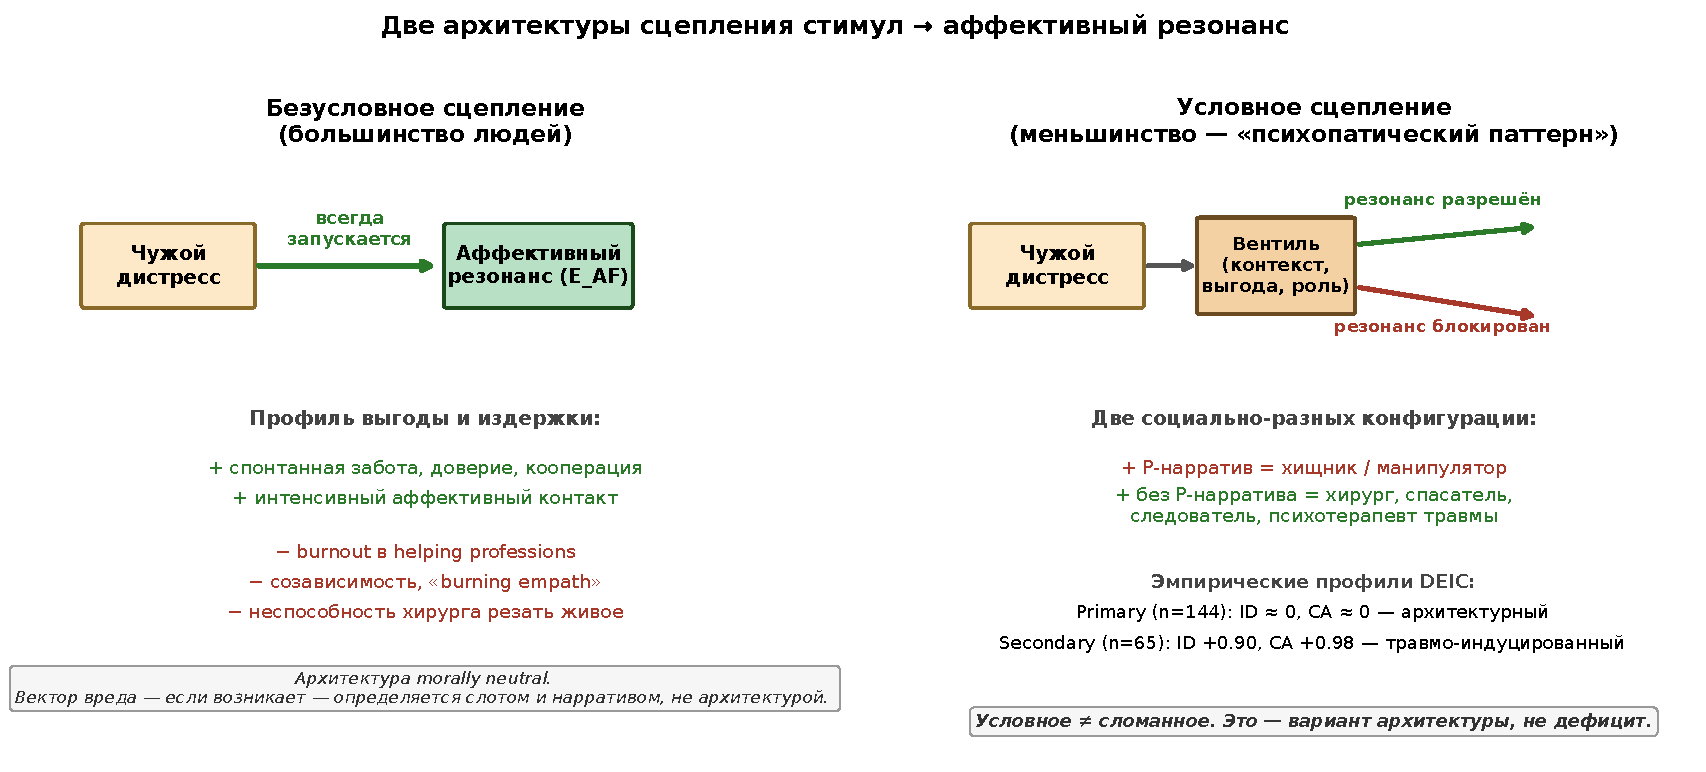
\includegraphics[width=0.95\linewidth]{figures/fig12_conditional_coupling.pdf}
\caption[Unconditional vs conditional affective coupling]{Architecture of \EAF{} coupling, not deficit. Left: \emph{unconditional} coupling --- affective resonance is triggered automatically, almost involuntarily, regardless of context and moral assessment (baseline pattern of the majority of the population). Right: \emph{conditional} coupling --- the same resonance is available but routed through a context-dependent gate; the combinations of this architecture with the P-narrative determine its social application. The empirical profiles of the primary ($n = 144$; ID $\approx 0$, CA $\approx 0$) and secondary ($n = 65$; ID $=+0.90$, CA $=+0.98$) cells are shown as two etiological trajectories into the conditional architecture.}
\label{fig:conditional_coupling}
\end{figure} Parallels in other functional systems help sustain the frame without a normative slide: people differ in the condition-sensitivity of the pain response, in autonomic reactivity, in the default level of arousal. None of these variations is labelled a malfunction by default --- each is evaluated in the concrete context of application.

Conditional coupling has an important double use that is usually crowded out of the clinical frame. In social roles that require working inside situations of suffering \emph{without} automatic affective entrainment, conditional architecture is not only compatible but functionally necessary. The surgeon who during an operation can stay cognitively precise while working with the living flesh and blood of a patient. The emergency physician who is effective in disaster precisely because affective resonance does not paralyse his actions. The investigator working with testimonies of sexual-violence victims. The trauma therapist sustaining many years of client states without burning out. Each of these roles requires \emph{conditional} access to affective resonance --- the capacity to turn resonance coupling on and off deliberately. Unconditional architecture in these roles yields high burnout vulnerability; conditional architecture gives stability. At population scale this variation serves functions that society otherwise could not fill.

This architecture becomes harmful only in combination with the \textbf{P-narrative} --- a stable moral claim ``this is permitted to me'' that turns conditional coupling toward deliberate instrumental use of others without moral obligation. This is precisely why \DEIC{} models P \emph{separately} from \EAF{}: the affective architecture in itself is morally neutral, and the moral narrative is an orthogonal layer that determines its social application. Conditional coupling without a P-narrative --- surgeon; conditional coupling with a P-narrative --- predator. Unconditional coupling with a P-narrative is an unlikely combination, rare in the data; unconditional coupling without a P-narrative is the baseline empathic pattern of most of the population, with its own vulnerabilities.

In our data this two-layer logic is visible in three empirical results. First --- \textbf{parallel mediation CA $\to$ \{ID, P, M\} $\to$ \EAF{}} in a unified model (§\ref{sec:results}.4.1): the CA $\to$ P path is essentially empty ($a$-coefficient $+0.015$, indirect effect 95\% CI $[-0.086, +0.060]$ includes zero), while the path via ID carries $\sim 173\%$ of the total CA effect on \EAF{}. At the population level P and CA are statistically orthogonal. This means the P-narrative is \emph{not} an adaptive consequence of childhood history but an architecturally independent layer. The secondary (hi-P-hi-CA) pattern is not ``P via CA'' but the co-occurrence of two independent axes in a subgroup of people. The primary (hi-P-lo-CA) pattern accordingly is not ``psychopathy without childhood trauma''; it does not belong to the same etiological line as the CA-mediated constructs at all.

The parallel-mediation result requires honest reconciliation with the unified SEM (§\ref{sec:results}.4.2), in which all paths --- parallel mediators, A main-effect on \EAF{}, and A moderation of both stages of the ID channel --- are estimated simultaneously. In that fuller specification the $a$-path CA$\to$ID remains robust ($+0.345$), CA$\to$P is still empty ($+0.011$, NS), but the $b$-path ID$\to$\EAF{} collapses to $-0.012$ (NS) once P is included in the same equation, while P$\to$\EAF{} dominates at $-0.726$. The moderation index \IMM{}, significant in the narrower specification of §\ref{sec:results}.4 ($-0.00197$, CI not including zero), also collapses to $+0.0001$ (NS) when P and A are present as predictors of \EAF{} in the same model. This is not a refutation of §\ref{sec:results}.4 and not an artefact of overfitting --- it is a re-composition of variance. At population scale the main explanatory weight on \EAF{} concentrates in the P channel (the ``permitted to me'' narrative) and in A main-effect (witnessing as an independent positive predictor of \EAF{}, $b = +0.393$), not in an isolated ID$\times$A moderation. At the clinical case level the cascade CA $\to$ ID $\to$ reduced \EAF{} remains substantively meaningful --- the $a$-path is real, ID as a mediator of traumatic experience in individual dynamics is present; but when we look at the whole sample, the direct negative predictor of affective empathy is not residual ID but the active P-narrative and (on the other side) active witnessing presence.

This refinement is important because it changes the clinico-theoretical formulation without losing the main content. We do not claim that the ID channel is absent. We claim: at the level of the whole population, the ID channel and the P channel share a substantial amount of variance in predicting \EAF{}, and in the unified model P carries the main weight (with its moral signature) alongside A (with its witnessing layer). This result strengthens rather than weakens the thesis of §\ref{subsec:architecture} about two-layer architecture: the architectural level (conditional/unconditional coupling) and the narrative level (P-permission) operate \emph{independently} of childhood history --- and their combination determines the social application of empathy far more strongly than residual ID dissonance on its own. ID is an important indicator of \emph{what is happening} inside a traumatized psyche; P is the decisive predictor of \emph{what this architecture unfolds into} at behavioral output.

Second --- separation of the primary and secondary patterns. Through a rule-based $2\times 2$ topological classification we identify the \textbf{primary pattern} ($n = 144$): conditional coupling without a traumatic history, with a pronounced P-narrative, without internal conflict (ID $\approx 0$, CA $\approx 0$). This is a configuration stable over time, not requiring a traumatic source --- an architectural variation onto which the P-narrative is ``superimposed'' as an independent moral structure \citep[in the terms of][empirically --- in similar proportions in \citealp{lilienfeld1990, patrick2010}]{karpman1941}. \textbf{Secondary pattern} ($n = 65$): conditional coupling with a traumatic history (CA $= +0.98$), with active internal conflict (ID $= +0.90$), with high Masking ($+0.63$). This is a configuration in which the conditional coupling mode is functionally \emph{forced} by the defensive system: automatic affective entrainment would be destructive, and the psyche has built conditional coupling as an adaptation. The P-narrative here usually remains active, but is structurally different --- it protects the remaining self rather than opening access to predation.

Third --- the distribution of A (attention) across groups and its interaction with architecture. The primary pattern has moderate A without special correlations with ID. The secondary pattern has low A ($-0.55$) --- its conditional coupling operates \emph{without} a witnessing relation, which makes it painful for the carrier. This points directly to different clinical entry points: the primary pattern has no ``wound'' that can be healed, and working with it is structural-social and narrative (restricting the P-narrative through external frames, where appropriate); the secondary pattern has a ``wound'' in the form of preserved ID, and A-work shifts conditional coupling into the integrated mode --- the same profile as the integrated survivor of §\ref{subsec:integrated_survivor}, but arrived at from a different history.

This is not a reproduction of the \emph{taxon} of \citet{hare2003} and not a claim that primary and secondary are different biological species. We claim more modestly: the architecture of conditional coupling exists in the population as a stable variation, etiologically it is reached by at least two paths (without trauma --- primary; via trauma as adaptation --- secondary), and the clinical interpretation ``psychopathy'' conflates these paths because at the behavioral level they look similar. They can be distinguished only through measurement of ID and CA. Without this distinction, therapeutic strategies systematically err: trauma-oriented interventions for the primary pattern land in emptiness; behavioral restrictive interventions for the secondary pattern ignore its internal conflict and potential resource.

The size of the secondary subgroup ($n = 65$) does not permit reliable effect-size estimates; this limitation requires a clinical sample for confirmation. But the direction of the distinction reproduces robustly in the latent topology and is not an artefact of any single index.

This reformulation --- architecture instead of deficit --- has consequences beyond the clinic. In the criminal-legal system, where psychopathy is often treated as a combination of moral and functional malfunction, separating architecture (neutral) from the P-narrative (morally significant) distinguishes what requires correction from what is not in principle subject to correction (architecture). In organizational psychology, the separation allows one to see that some roles require conditional architecture and that its ``treatment'' runs against function. In public communication, it allows one to stop speaking of psychopaths as ``broken people'' and move to a conversation about a combination of capacities and narratives that society can regulate through external structures, rather than through attempts to remake the inner architecture.

\subsection{Positioning: elephant, not master-map}
\label{subsec:positioning}

We deliberately choose a positioning that differs from most integrative psychological projects. \DEIC{} does not claim to be ``the first unified framework of empathy'', ``the resolution of the dispute between psychoanalysis and neuroscience'', ``the integration of all traditions''. We choose a narrower and more defensible position: \DEIC{} is a \emph{compression}, not a \emph{summation}. Different traditions (psychoanalytic, attachment theory, cognitive neuroscience of empathy, mirror-neuron literature, clinical tradition of psychopathy from Cleckley to Hare, contemplative traditions of witnessing) really do touch the same subject in different ways, and each touch is real. Our contribution is that we measured six distinguishable functions in \emph{one} sample, showed their stable structural relations, and thereby made visible the \emph{joints} between what these traditions describe separately.

We deliberately do not take the position that \citet{wilber1995, wilber2000} took toward the traditions. Wilber asserted that there exists a \emph{super-map} (AQAL: four quadrants $\times$ levels $\times$ lines $\times$ states $\times$ types), on which every tradition occupies its hierarchically determined place. This is an ontological claim: the map is primary, the traditions secondary, and each sees only a fragment of the whole that the meta-theorist sees. In our work four real differences from this position are important and will be maintained as discipline, not stylistics.

First, level of claim. Wilber constructs an ontology --- a meta-metaphysical claim about how reality is organized. \DEIC{} constructs a measurement model --- a psychometric model of six functions on a concrete sample. The first is irrefutable by construction; the second must reproduce in new samples, and if it does not reproduce, it is refuted.

Second, hierarchy of coordinates. In AQAL levels are hierarchical and normative: integral $>$ pluralistic $>$ rational $>$ mythic $>$ magical $>$ archaic. In \DEIC{} the six coordinates are non-hierarchical. There is no preset position that ``high A is better'' or ``low P is better''; there are empirical correlations with outcomes, but these are consequences of data, not normative judgments. The ``integrated survivor'' is one profile among many, not a summit.

Third, relation to traditions. Wilber assimilates: each tradition gets a place on \emph{his} map, and its internal structure is reinterpreted through AQAL. \DEIC{} does not place traditions. We say: ``the construct X we measured correlates with what tradition A calls \textit{sākṣī}, what tradition B calls \textit{rigpa}, what tradition C calls self-remembering''. These descriptions within their own systems are autonomous. We do not embed the systems into \DEIC{}; we show where a psychometric coordinate of \emph{our} model correlates with what they describe.

Fourth, modesty about the not-understood. Wilber explains everything, including internal contradictions --- they are assimilated as ``a lower level looking at a higher one''. \DEIC{} has an explicit list of what it does not explain (see §\ref{sec:limitations}, §\ref{sec:future}): temporal scaffolding, mechanism of switching between ID and P, mechanism of the therapeutic force of A, individual differences in A-trainability, developmental branching in the $2\times 2$, evolutionary-ecological substrate, reflexivity of the observer. This is not a defect --- it is a boundary.

A short formula that will recur several times in this section: Wilber --- ``I see the whole; the traditions see parts of my map; you are now at level X''; \DEIC{} --- ``I see six measurable functions. Some traditions describe one of them more deeply than we do. The coordinate scaffolding is not metaphysics but statistics; it can and should be refuted.''

\subsection{The anti-Wilber discipline: hygiene of language}
\label{subsec:discipline}

The position of §\ref{subsec:positioning} is enacted through a set of disciplinary rules that must be satisfied in every paragraph. First rule --- every claim about a construct is accompanied by a falsifier. If we write ``A moderates the CA$\to$ID$\to$\EAF{} channel'', we are obliged to add: ``if in pre-registered replication the \IMM{} 95\% CI includes zero, this claim is refuted''. By this we distinguish \DEIC{} from systems that explain everything (and thereby explain nothing).

Second --- ban on hierarchy between factors. We do not write ``A is maturity'', ``integrated survivor is the highest point'', ``witnessing is a more developed level''. We write ``empirically linked to [concrete result]''. This may seem pedantic, but it is precisely at this point that most meta-theoretical projects slip off the rails: normative language is embedded invisibly and closes the path to empirical verification.

Third --- do not assimilate the traditions, but do not keep them at a symbolic distance either. We do not write ``Zen is about A''. We write ``Zen describes a similar construct in its system; its correlation with our model is such and such''. If we cannot make the second part of the statement, we do not make the first. At the same time we \emph{do} make the second part --- and we make it at length, when a tradition supplies an operational distinction that the psychometric literature has not yet reproduced. Cultural references (advaita, dzogchen, Fourth Way, contemporary non-dual, McKenna) in \DEIC{} are not decorative ornament and not a display of academic boldness at the expense of rigor; they are sources of hypotheses that we either formulate as falsifiable or omit without mention. The Bayesian prior on divergence between our data and a contemplative tradition is ``we have not yet measured what they distinguish'', not ``they were wrong''.

Fourth --- measurement model $\neq$ ontological claims. We do not write ``\DEIC{} describes the psyche''. We write ``\DEIC{} is a psychometric model of six functions on an $N = 1426$ Russian-language online sample''. This restriction of the claim protects us from turning into a meta-theory.

Fifth --- lexical discipline. \emph{Extends, operationalizes, is consistent with, replicates within our framework, provides psychometric coordinates for} --- allowed. \emph{Unifies, completes, first to integrate, resolves, supersedes, subsumes} --- forbidden. The choice of verb in a key claim of the program is the choice between serious work and meta-theoretical pretentiousness.

Sixth --- an obligatory ``what \DEIC{} does not explain'' section of visible size, not in a footnote (see §\ref{sec:limitations}--\ref{sec:future}).

Seventh --- reflexivity clause: the methodological paper of the program will contain an explicit section on the fact that the observer (researcher) with her own level of A affects what she is capable of measuring in the observed. This is a structural epistemological acknowledgment, not a mystical remark.

\subsection{Falsifiability as a structural level}
\label{subsec:falsifiers}

The generative character of the model is more important than its descriptive character. All predictions formulated in the previous subsections of the Discussion --- two-stage A-moderation of the CA$\to$ID$\to$\EAF{} channel, collapse of the $b$-path ID$\to$\EAF{} in the unified SEM, CA$\perp$P orthogonality at the population level, distinguishability of primary and secondary psychopathy, the \EAF{} effect in the integrated-survivor cell, hyper-instrumentation P$\to$\Ecog{}, and others --- are moved to a separate structural section (§\ref{sec:falsification}) in the form of claim/falsifier pairs with explicitly stated test requirements and consequences of refutation. That section is not an extended commentary on the Discussion; it states \emph{at exactly which observations} the claims of this paper should be considered false. For reading the Discussion this means: all claims in the findings register (``the data show'', ``the model yields'') have scientific status exactly to the extent to which §\ref{sec:falsification} formulates their falsifier. That section is not an appendix to the paper but the condition on which the paper belongs to the empirical genre rather than the rhetorical one.

\subsection{Relation to existing theories}
\label{subsec:relation_to_theories}

\DEIC{} is compatible with most of the main lines of research on empathy and psychopathy, but diverges from dominant interpretations at a number of points. We do not claim these lines are wrong wholesale; we point to places where our model departs from them.

\citet{baroncohen2011} --- EQ as a dispositional trait: in our model \EAF{} is a state regulated by A; the trait model misses the core of the mechanism. ``Psychopaths lack cognitive empathy'' --- a popular oversimplification; our partial correlations show the opposite: $r$(P, \Ecog{}) $= +0.32$ after partialling. Cognitive empathy in psychopaths is often \emph{elevated}; it is precisely this that makes ``predation'' possible, as described by \citet{blair2013} and \citet{baroncohen2011} under the heading of hyper-instrumentation. Hare's taxon-view of psychopathy --- we find no categorical kinds in our data. A dimensional model with two orthogonal etiologies describes the topology of our results more accurately. \citet{newman2003} response-modulation theory as a universal explanation of psychopathy --- in our P patterns cognitive attention is intact; the witnessing-affective coupling operates in a \emph{conditional}, not an unconditional, mode. Response-modulation captures part of this mechanism --- selectivity of attention --- but does not separate the architectural layer (conditional coupling, morally neutral) from the narrative layer (P-permission).

Classic attachment determinism \citep{bowlby1969} in its simplified reading: CA $\to$ dysfunction linearly. Our data show moderation through A. Determinism is false; compensation is empirically real. \citet{vaillant1977} hierarchy of mature vs immature defenses --- we do not find that defenses per se are pathological. ID without A yields dysfunction; ID with A --- functional compensation. The moral frame ``mature defense better than immature'' turns out to be less informative than the frame ``defense plus witnessing''.

NICE/APA CBT-first for all mood disorders \citep{nice2022, apa2019}. \DEIC{} directly predicts that in high-ID / low-A clients CBT lands in resistance or yields superficial improvement without change in the underlying mechanism. Self-reported psychiatric dx count as a severity measure --- our data show that ID blocks help-seeking, so dx\_count \emph{underestimates} the heaviest cases. FFMQ \citep{baer2006} as an operationalization of mindfulness --- our A-CFA empirically demonstrates that metacognitive items conflate attention-to-internal-states with witnessing. We support the critique of \citet{vandam2018}. \citet{wilber1995, wilber2000} AQAL --- we do not reproduce hierarchical-stage models of the development of consciousness in our data. We do not find stages; we find distributed non-hierarchical coordinates.

\subsection{ACE extension: ``don't remember'' as part of the construct, not as missingness}
\label{subsec:ace_extension}

The standard operationalization of adverse childhood experiences, descending from \citet{felitti1998} and established in the CDC/Kaiser line and in virtually all of the derivative corpus, admits two legitimate responses per ACE item from the respondent: ``yes'' (the event occurred) and ``no'' (it did not); everything else---``I don't remember,'' ``I am not sure,'' a refusal---is treated as missing data, excluded, or imputed. ACE items meanwhile ask not about emotional interpretation of childhood but about \emph{facts}: whether a parent was incarcerated, whether substances were used in the family, whether domestic violence occurred, whether a parent died, whether the parents divorced. To a factual question, ``I don't remember'' has, at the population level, exactly two substantive interpretations, and \emph{neither of them reduces to statistical missingness}. First: the respondent was not told---which is itself a marker of a family pattern of silencing around a high-adversity environment (families that systematically discuss a deceased parent or an episode of violence produce different respondents than those that answer ``don't remember''). Second: the respondent dissociated---which is a direct behavioral manifestation of the very defensive mechanism D that the ID latent measures at the other end of the instrument. Both interpretations are ACE-relevant; both are empirically opposite to treating ``don't remember'' as missing. The standard coding in that case \emph{excludes from analysis precisely the sub-contingent in which the ACE signal should be strongest}. This is not a minor coding detail but a structural undercount in the standard ACE methodology, inherited by the whole corpus.

The DEIC construct proposes an extension: ``don't remember'' on an ACE item should be treated as a \emph{positive signal of an adversity-relevant family or cognitive configuration}---either of family silencing or of a dissociative encoding gap---and coded numerically on par with ``yes.'' ACE then ceases to be a one-dimensional event counter and becomes two-layered: an explicit count of confirmed events plus a count of ``don't remember'' responses as a separate ACE-dissociation subscale.

Empirical validation of the extension was obtained on the present sample through a full re-fit of the 6-factor oblique CFA in which the canonical code ``don't remember''~$=$~NaN was replaced with ``don't remember''~$=$~1. Of 1470 respondents, 667 (45.4\,\%) used ``don't remember'' at least once across the 10 ACE items; 294 (20\,\%) used it twice or more. Under the extended coding, N passing the $\le 10\,\%$ missing filter rises to 1468 (vs. the canonical 1426); mean ACE count shifts from 3.43 to 4.18; MLR-robust CFA retains acceptable fit (CFI~$=$~0.960, TLI~$=$~0.949, RMSEA~$=$~0.062 against canonical 0.950, 0.936, 0.068; df~$=$~120 in both cases). Latent correlations in the 6-factor oblique model shift in the direction consistent with the DEIC hypothesis: $r(\text{CA}, \text{ID})$ rises from $+0.668$ to $+0.712$; $r(\text{CA}, \EAF{})$ strengthens in magnitude from $-0.129$ to $-0.205$ ($+59\,\%$); $r(\text{CA}, M)$ rises from $+0.195$ to $+0.267$; while $r(\text{CA}, P)$ remains weak (rising from $+0.015$ to $+0.122$---still within the ``weak'' range), preserving the architectural orthogonality of P to childhood adversity.

Parallel mediation CA~$\to\{$ID, $P$, $M\}\to\EAF{}$ on latent scores in split-B, under canonical and extended coding with 5{,}000 bootstrap draws, yields a consistently strengthened picture. The total effect $c$(CA~$\to$~\EAF{}) strengthens in magnitude from $-0.129$ to $-0.205$. The indirect effect through ID---the canonical ``defense kills empathy'' channel---retains its structure: $-0.223$ [$-0.267, -0.181$] under canonical coding, $-0.236$ [$-0.282, -0.192$] under extended; the CI excludes zero in both cases. The indirect effect through P \emph{becomes statistically distinguishable from zero} precisely under the extension: canonical $-0.014$ [$-0.086, +0.060$] (NS), extended $-0.140$ [$-0.234, -0.048$] (statistically significant). This does not redefine the architectural orthogonality of P to CA as a population fact, but it indicates that part of the P channel had been instrumentally under-detected precisely where respondents had engaged dissociative encoding of childhood. The direct effect $c'$ (CA~$\to$~\EAF{} controlling for ID, P, M) remains positive under both codings ($+0.073$ canonical, $+0.048$ extended); that is, the headline sign flip of the principal mediation conclusion---``trauma damages empathy via the defense, not directly''---is robust to the coding of ``don't remember.'' No 95\,\% bootstrap interval of the originally significant indirect effects crosses zero under the extended coding; the shifts are numerically detectable rather than noise.

The operational implication for wave 2: ACE items retain a three-option format ``yes / no / don't remember,'' but ``don't remember'' is coded as a positive signal; the counter of such responses across all 10 items is constructed as an independent ACE-dissociation subscale. Psychometric prediction: at $n \ge 300$, this subscale should yield McDonald's $\omega \ge 0.7$ and correlate positively with the ID latent ($r \ge 0.30$ at the latent level); when it is controlled, the association of the ``explicit'' ACE count with ID should attenuate, which provides a formal test of the subscale's validity as a distinct channel. The conceptual implication is broader. We do not claim a generalization of \emph{effect sizes} to the entire ACE literature---that would require a meta-analytic re-fit; we point to a \emph{structural} problem in the coding logic inherited by the whole corpus \citep{felitti1998}. Wherever that logic is identical, the directional meaning-constructing shift is identical: any self-report of sensitive information from early life---sexual history, substance history, family secrets---in which ``don't remember'' is a legitimate and socially acceptable response, requires explicit modeling of that response as a construct-relevant signal, rather than mechanical reduction to missing. See §\ref{sec:future} for the wave-2 design and §\ref{sec:limitations} for the boundaries of the present estimate.

\subsection{Declarative--behavioral asymmetry (DI) as a signal of architectural fragmentation}
\label{subsec:di_asymmetry}

The pilot composite version of the instrument (DEIC-DRAFT, August 2025) was built on the principle of paired formulations: each content item existed in a declarative register (abstract self-description: ``I am an empathic person,'' ``I manipulate others,'' ``I suppress my emotions'') and a behavioral register (a concrete narrow-window behavioral report: ``yesterday I stopped and really listened,'' ``last week I hid an important detail from my partner for my benefit,'' ``this morning I refrained from showing irritation''). The summary index $DI = \overline{\text{decl}} - \overline{\text{beh}}$ across all items in the pilot showed a statistically significant population shift ($p < 0.001$, $d \approx 0.43$), with the leading contribution from the AIS scale (declarative 5.04 vs. behavioral 3.35). On this basis DI was described in the pilot report as an independent indicator of social desirability. Below we show that this description was partially wrong: the population shift replicates, but across scales it is bidirectional, and what DI actually measures is not a uniform self-presentation distortion but an \emph{architectural gap between abstract self-schema and episodic behavioral recall}.

On the main sample ($N{=}1470$) the declarative--behavioral gap was computed across eight scales with sufficient paired-item balance (ADI, CA, D, EC, Empathy, Psychopathy, Suppression, Masking; 38 declarative against 40 behavioral). Paired $t$-tests are significant on all eight scales, but the distribution of $d$ in magnitude and direction differs substantially. Positive DI (declaration exceeds behavior)---E ($d{=}{+}0.44$), EC ($d{=}{+}0.45$), ADI ($d{=}{+}0.20$), CA ($d{=}{+}0.19$). Negative DI (behavior exceeds declaration)---P ($d{=}{-}1.05$; the largest effect on the sample), MS ($d{=}{-}0.30$), S ($d{=}{-}0.10$), D ($d{=}{-}0.09$). The summed raw DI turns out to be weakly negative ($d{=}{-}0.11$)---the sign of averaging oppositely directed scales. If DI is aligned in the prosocial direction (for stigmatized scales the sign is reversed, so that $+$ always means ``I pass declaratively as a more positive version of myself than my behavior shows''), the shift becomes uniformly positive: $d_{aligned}{=}{+}0.29$, 95\,\% CI $[{+}0.14, {+}0.20]$. The pilot observation therefore replicates, but as a \emph{joint outcome of two different mechanisms} rather than as a uniform social-desirability bias.

Disentangling these mechanisms is the principal substantive result of this subsection. For stigmatized scales with explicit self-incriminating content (P, MS, S, D), narrow-focus behavioral items (``this week I \ldots'') collect more admissions than declarative trait descriptions---what the respondent is unwilling to own as a trait, they are willing to acknowledge as an episode. This is most vivid on P: the pair $P_4$ (``I manipulate people to get what I want'') vs.\ $P_{\text{new\_3}}$ (a concrete behavioral description of an exploitative situation within the preceding period) yields a mean gap of $-2.66$ points on a 7-point scale ($d{=}{-}0.98$); that is, the respondent systematically denies the trait schema of psychopathy but clearly recognizes concrete manifestations of it in their own behavioral archive. This reproduces at an operational level a long-standing clinical observation about the split between trait identification and episodic behavioral self-report under a psychopathic narrative \citep{hare2003, lilienfeld1990}. For desirably valenced scales (E and, with a qualification, EC), the direction is opposite: the trait schema is broad, the behavioral episode is narrow---the respondent holds a developed self-presentation as empathic, supported by a wide history, while a concrete narrow-window behavioral item (``this morning I \ldots'') does or does not land in a specific behavioral episode. For shared-adversity scales (ADI, CA) a positive gap points to the opposite pattern: the trait level partially overstates an inner history that the concrete behavioral episode in ordinary life does not confirm---a possible methodological consequence of ADI- and CA-declarative items querying a global affective self-concept not tied to recent code.

That DI does not reduce to social desirability is confirmed by its connections with the latent architecture. $DI_{overall}$ (raw, undirected) correlates with ID as $r{=}{+}0.590$, with CA as $r{=}{+}0.580$, and with A as $r{=}{-}0.517$; with the clinical diagnostic variable ($\text{dx\_free\_text\_any}$)---$r{=}{+}0.017$ (NS, $p{=}0.66$). In other words, the magnitude of the declarative--behavioral gap tracks the \emph{internal fragmentation between the trait-self-schema layer and the episodic-behavior-recall layer}, and this fragmentation is marked by the same architectural latent (ID) that elsewhere in the work is registered as the defensive contour. $A$ as a witnessing function narrows the gap. Clinical status plays no role here, which is structurally consistent with §\ref{subsec:architecture} and §\ref{subsec:free_will}: DI is an architectural, not a diagnostic, metric. $DI_{aligned}$ (rotated in the prosocial direction) gives a mirror image: $r(DI_{aligned}, A){=}{+}0.658$, $r(DI_{aligned}, \EAF{}){=}{+}0.550$, $r(DI_{aligned}, ID){=}{-}0.645$, $r(DI_{aligned}, P){=}{-}0.362$. Under a median split on $A$, the contrast of $DI_{overall}$ between low-A and high-A yields $d{=}0.90$ (tertile contrast $d{=}1.22$); the $A$-field fully restructures the direction and magnitude of the gap.

A separate finding concerns $piz$---the integral metric implemented in the instrument for tracking facade work (masking + lie; §\ref{subsec:integral_metrics}). $piz$ and DI are structurally and empirically distinct. $r(piz, DI_{overall}){=}{+}0.198$ (small positive), $r(piz, DI_{aligned}){=}{-}0.274$---that is, $piz$ and $DI_{aligned}$ diverge even in sign (higher masking $\Rightarrow$ \emph{smaller}, not larger, prosocial shift of declaration over behavior). On individual scales $r(piz, DI_{P\_scale}){=}{+}0.359$: higher masking is associated with a more pronounced $\textit{beh}>\textit{decl}$ gap on the P scale (high facade work amplifies precisely the asymmetry in which trait denial goes hand in hand with behavioral acknowledgment). In sum: $piz$ measures self-presentational pressure, $DI$ measures structural fragmentation---two distinct layers, both operationalizable.

For instrument infrastructure this means that $DI$ should be recorded alongside $piz$ as a sixth \texttt{extended\_metric} in \texttt{psychometrics.json} (with per-scale and overall-aligned versions). For the theoretical frame it means that the pilot observation is recovered, but in a substantively refined status: it supplies an operational psychometric grid for the long-standing psychoanalytic distinction between the ``ideal self'' as trait-schema and the ``acting self'' as behavioral archive \citep{freud1917, winnicott1965}, where the gap between them is not a measurement defect but a substantive marker of architecture. The methodological implication for wave 2: any psychometric scale claiming a diagnostic function in the $ID$/$P$/$E$ domains must include paired declarative and behavioral formulations, because it is their gap, rather than either formulation in isolation, that provides access to the architectural layer.

\subsection{\DEIC{} and the theory of consciousness: the boundary at which we work}
\label{subsec:consciousness}

\DEIC{} does not offer a theory of consciousness. The hard problem \citep{chalmers1995} is a boundary that psychometrics does not cross and must not pretend to have crossed. We measure functions \emph{within} consciousness (attention, dissonance, empathy); we claim nothing about the nature of subjective experience as such, and this restriction is serious, not rhetorical.

But from the reality of the boundary it does not follow that one should keep distant from it. On the contrary: it is precisely near this boundary that the most substantive interface of empirical psychometrics with contemplative studies arises. A is the psychometric trace of what various traditions single out as a structurally different layer of consciousness: \textit{sākṣī} in advaita, \textit{rigpa} in dzogchen, ``self-remembering'' in Gurdjieff, non-dual awareness in the contemporary non-dual literature. We do not explain what the witness is. We show that witnessing is measurable, functional, and that its action on the CA$\to$ID$\to$\EAF{} channel reproduces in the narrow specification. This makes A the point at which psychometrics \emph{comes into contact} with the part of consciousness usually treated as non-functional --- without assimilating it and without claiming its nature, but without skirting it either.

The sharpest dialogue of this type is with \citet{mckenna2002, mckenna2004, mckenna2013}. In most Western representations of contemplative traditions, awakening is described additively: more awareness, more acceptance, more presence. McKenna inverts this. His thesis is \emph{spiritual autolysis}: awakening is a destructive process, the dissolution of illusory structures, not the accretion of new capacities. More attention does not bring consolation; it reveals the constructedness of one's own states and of the world, and this revelation is not pleasant. The ordinary person avoids it, because there is no consoling frame there.

In the \DEIC{} frame McKenna's thesis becomes a direct longitudinal prediction. In people going through intensive retreats with deep witnessing practice, A rises. If McKenna is right, over a short time-interval ID \emph{rises} --- the revelation of constructedness produces temporary destabilization of identity, which is precisely the signature that in our cross-sectional model we read as dissonance. The trajectory then branches: either regression (defenses return, A falls back, the destabilization closes through the usual structure), or integration (acceptance of constructedness, a profile topologically corresponding to the integrated survivor of §\ref{subsec:integrated_survivor}, but arrived at not through childhood trauma but through a voluntary practical path). This is not a prediction of ``is McKenna right''; it is the operationalization of his thesis in a form that can be refuted by longitudinal data on retreat cohorts.

This is our position relative to the theory of consciousness. Not to replace it, not to claim its territory --- but not to make its existence an excuse to avoid contact either. Work at the boundary is possible and necessary: making concrete psychometric predictions at points where contemplative traditions hold operable distinctions that empirical psychology is only beginning to capture.

\subsection{Clinical implications}
\label{subsec:clinical}

The model has several concrete clinical implications, which we formulate as \emph{proposals for testing}, not as recommendations for immediate adoption.

\paragraph{Work with A before work with content.} In clients with high ID and low A a direct cognitive intervention often lands in resistance or yields superficial improvement. Our model predicts that the sequence ``A-work $\to$ content-work'' will be more effective than ``content-work without prior A''. This formalizes what somatic experiencing \citep{levine2015}, sensorimotor psychotherapy \citep{ogden2006}, IFS \citep{schwartz1995}, mentalization-based therapy \citep{fonagy2008}, and a range of psychodynamic approaches do intuitively. A pre-registered RCT with baseline A and ID as moderator of treatment effect is a direct test.

\paragraph{Distinguishing primary and secondary patterns in clinical assessment.} Without measuring ID and CA the two patterns look identical but require different strategies. Primary --- conditional architecture without a ``wound'': clinical work with the architecture as such is useless and may even be inappropriate (in functional social slots this architecture gives stability); work with the P-narrative through external frames is appropriate when the narrative turns predatory. Secondary --- work with trauma and expansion of A, aiming to shift the preserved ID into integrated mode.

\paragraph{A-training as the central component of long-term work.} Our model predicts that non-dual mindfulness practice will yield a stronger effect on \EAF{} recovery than behavioral mindfulness in the MBSR style. This formulates a head-to-head testable comparison.

\paragraph{Burning empath as feed-forward risk.} The profile CA + hi \EAF{} + lo A should predict burnout in helping professions.

\paragraph{Substance use as phenotype, not cause.} In the subgroup of blocked-sober-high-P the same P/D/ACE profile is observed as in active substance users. This indicates that substance use is an \emph{exit} from blocking, not its source. A-training in work with addictive behaviors should give a stable effect where abstinence-based programs relapse.

\paragraph{A therapist with low A does not see the client's ID activation.} This has a direct clinical consequence: supervision and self-work of the clinician are not a ``nice to have'' but a structural condition of the possibility of seeing what is happening in the client.

\subsection{Free will as a gradient of attention}
\label{subsec:free_will}

One of the most conceptually heavy consequences of \DEIC{} is a reformulation of the problem of free will. We do not claim to solve it. We claim that in its classical binary form --- ``is the will free?'' --- it is posed at the wrong grain and therefore has no answer. At the grain our model provides, it decomposes into a concrete empirical question: \emph{what is the magnitude of A in a given situation for a given agent?}

In \DEIC{} coordinates, behavior can be read as the result of interaction between two layers: the automatic D/P/E configuration (what triggers in response to a stimulus without participation of a witnessing relation) and A (the gap between trigger and action, in which a different distribution of attention, a different relating, a different reaction becomes possible). A low-A agent at a given moment is functionally determined by her configuration: the stimulus activates the channel, the channel unfolds automatic behavior, observation is absent. A high-A agent at the same moment has a \emph{measurable gap} between activation and action, within which a different trajectory is possible. This is not a metaphysical distinction but an empirical variable --- the same one our A-moderation fixes in the narrow specification: at high A the CA$\to$ID$\to$\EAF{} channel flips sign precisely because A wedges between the habitual trigger and its habitual outcome.

Philosophers who asked about free will approached the same gradient from different sides. Augustine's ``slave of the will'' and his description of \textit{liberum arbitrium captivatum} is a description of the low-A state, in which desire continuously unfolds into action without a gap. Kant and his primacy of practical reason --- a description of a function that appears at high A: the \emph{Maxime} as a conscious principle of conduct, not an impulse. \citet{libet1985} with his early readiness potential and the critics of his interpretation \citep[see][]{frith2008} point out that a voluntary act does sometimes lag behind brain activity, but the \emph{veto function} remains --- this is A, holding the gap. \citet{frankl1946} --- ``between stimulus and response there is a space; in that space our power lies to choose our response'' --- a direct description of A-moderation in clinical language. Buddhist \textit{vīmaṃsā} (investigative attention) and \textit{yoniso manasikāra} (wise attention) describe practices that build A as the condition of ethical possibility; the advaitic distinction between \textit{vṛtti} (movements of mind) and \textit{sākṣī} (the witness) --- the same structural asymmetry. Gurdjieff's ``man-machine'' is a description of the low-A mode, and ``self-remembering'' is an operational protocol for raising A. When these lines converge on the observation that the ordinary person acts out of automatism most of the time, and that moments of freedom are tied to a special quality of attention, they converge non-accidentally --- they describe the same measurable phenomenon in different languages.

From this reading a series of predictions follows. First, the agent's perception of his own voluntary act as ``free'' should correlate with his momentary A, not with his trait-level self-efficacy or with the narrative of self-determination. Paradigms of the \citet{westgate2019} meaning-in-action type can be reframed as A-assays. Second, interventions that raise A (non-dual mindfulness, somatic work, psychedelic integration) should produce measurable growth in variables usually associated with self-determination: intrinsic motivation, moral consistency, capacity to forego short-term reward for a long-term value. Third, populations with systematically suppressed A (see §\ref{subsec:political}) should display systematically reduced functional freedom of choice --- not as a moral defect but as a direct consequence of the destruction of the operational infrastructure of freedom.

The ethical consequence of this reading is not the abolition of responsibility but its structural recalibration. The question ``was he free in that moment?'' acquires an empirical answer: what was his A-configuration at the moment of action, what was the variance of his A over time, what is the trajectory of its development. Responsibility is preserved but distributed differently: for a concrete act at a low-A moment --- lower in intensity than for the long-term trajectory of care for one's own A infrastructure. This coincides with the intuition that clinical common sense and a number of legal systems already use de facto (mitigating circumstances, diminished capacity, forensic assessment of the state at the time of the act), but makes it operational. Forgiveness, which in most traditions is formulated ethically (``forgive them, for they know not what they do''), becomes an epistemologically correct attribution: at a low-A moment the agent did not know, because the infrastructure of knowing was not deployed.

We stress that this does not abolish the difference between acts produced out of low-A automatism and acts produced with A support from a pronounced P-narrative. The former are structurally unfree, and standard therapeutic and educational work is, as a rule, the adequate response. The latter are architecturally different: high A, holding the P-narrative ``this is permitted to me'', is not the absence of freedom, but a choice out of high A in favour of violation. The social and legal response to these two classes of acts must be structurally different, and \DEIC{} supplies a coordinate grid in which such a distinction can be made operationally, not impressionistically.

\subsection{Politics, media, attention: \DEIC{} at social scale}
\label{subsec:political}

The outputs of \DEIC{} beyond individual clinic require a separate discussion. We formulate them as \emph{theses for discussion for future research programs}, not as ready policy recommendations. The link between the architecture of individual psyche and social patterns is not direct, and every claim at the social scale on the basis of an $N = 1426$ Russian-language online sample is a hypothesis, not an established fact. But it is precisely because \DEIC{} contains explicit operational coordinates that these hypotheses can be formulated so that they can be tested.

\paragraph{Political demagoguery as a P$\times$low-A market.} A political style that the literature describes as populist/demagogic has, in \DEIC{} language, a clear signature on the leader's side: high P (the moral narrative of permission --- ``I lead them, I am allowed to decide for them''), moderate conditional \EAF{} (enough for ritual performance, not paralysing action), and --- \emph{crucially} --- high \Ecog{} (instrumental understanding of the audience). This is not an ad hominem attribution to concrete politicians --- it is a description of the structural niche which, in a population with low A, becomes socially adaptive and selectively preferred. \citet{westen2007, haidt2012} show that audiences vote not so much rationally as through moral and identificatory circuits; our framework sharpens this: audiences with low A-infrastructure choose not ideas but moral narratives that coincide with their own unreflective self-concept. Prediction: electoral support for P-style demagoguery should be predictable not by socioeconomic markers as such, but by the general A-level of the audience at the time of the election.

\paragraph{Attention economy as a structurally psychotogenic environment.} If A is the structural condition of integration and therefore the condition of the possibility of a stable psyche (see §\ref{subsec:integrated_survivor}), then an environment systematically destroying A acts as a psychotogenic agent at population level. Contemporary engagement-optimized media systems are structurally such an environment. The mechanism is three-layered: (a) fragmentation of A through micro-interruption (notifications, continuous feed, swipe interfaces), (b) surfacing of P-content as an engagement maximum (outrage, moral indignation, identity signaling), (c) delivery of consoling D-content (echo-chamber confirmation of the existing defensive configuration). In sum: simultaneous decline of A, growth of P-patterning in mass communication, stabilization of D. This is a reading of the observed ``epidemic of anxiety/ADHD/polarization'' not as an epidemic of separate disorders, but as a single structural degradation of the \DEIC{} configuration in the population. Concrete testable predictions: (i) intensity of use of engagement-optimized platforms predicts a decline in A in 6--12-month longitudinal studies; (ii) adolescent cohorts with early exposure to algorithmically-curated feeds have a measurably different \DEIC{} topology than cohorts with the same ACE load but without early exposure; (iii) experiments with attention-protective design (edit-mode, pause interfaces, slow-feed) should yield a measurable gain in A, other things equal.

\paragraph{Democracy as an A-dependent institution.} We formulate this cautiously, because a claim of this scale requires data of correspondent scale. Nonetheless: if democratic participation structurally presupposes the capacity to hold a complex moral and cognitive object (a political decision) long enough to deliberate on it --- that is, presupposes A --- then democracy in an environment of systematic A-destruction cannot sustain its own function. This is not an argument against democracy; it is an argument that democracy has historically rested on an attention-protective infrastructure (church, education in its older form, slow media, communal institutions) which secularization and commercialization have not replaced with an equivalent. The result is a regression of politics into populism, polarization, high susceptibility to P-style. The practical consequence: investments in attention-protective institutions --- educational reform, a contemplative component in general pedagogy, regulation of engagement-optimization as a public health issue --- are structurally necessary for sustaining democratic function. This thesis cannot be directly tested on our sample, but it follows logically from the A-moderation of individual functioning we have found.

\paragraph{Cults, authoritarian movements, sectarian politics.} The frame allows the dynamics of cults and authoritarian movements to be read in a single logic: the leader carries the dominant P-narrative of selectedness or exclusivity; followers bring D and low A --- a search for external structure that will dispense with the need for independent observation; the cult provides apparent integration through external structure instead of inner A-development. This reading makes the reintegration work with ex-cult members and ex-radicalized persons not simply cognitive deradicalization, but restoration of the A-infrastructure the movement suppressed. Empirically testable: \DEIC{} profiles of people leaving cultic/authoritarian movements should be characterized by low A and a D profile preserved in a frozen form; long-term therapeutic work should be accompanied by growth of A and the release of held D-content.

\paragraph{Collective D and transitional justice.} Post-genocide, post-totalitarian, post-colonial societies carry a collective analogue of individual D configuration: systemically suppressed, affectively unintegrated relation to their own historical reality, transmitted transgenerationally \citep{yehuda2015, meaney2001}. \citet{herman1992} in her formulation of complex trauma points to the collective layer; our framework makes measurable the assumption that transitional justice (truth commissions, memorial practices, public historical reckoning) works precisely as collective D-work --- and thus is effective where it opens space for affective integration, and ineffective where it is reduced to a procedural legal form. The Russian-language sample on which our model is validated carries an elevated baseline CA/ID densely connected with two twentieth-century wars, repressions, and the nineties; we hypothesize (and await cross-cultural replication) that this is not cultural noise of the sample but a measurable collective D configuration reflected in individual psyche.

\paragraph{Religions, secular substitution, collective A-infrastructure.} We describe this as a thesis for discussion, seeking to stay equally distant from religious apologetics and secular dismissal. Empirically: the major religious traditions historically contained three functional components systematically working with \DEIC{} configuration --- A-training (prayer, meditation, ritual examen), D-aperture (confession, collective lament, ritual mourning), P-restraint (commandments, examination of conscience). Secular contemporary substitutes (therapy, wellness industry, philosophy of practical life) try to reproduce part of these functions in individual voluntary form, but without institutional-level continuity and without collective infrastructure. Forecast: secular societies must \emph{rebuild} the equivalent of a collective \DEIC{}-calibration infrastructure or accept the epidemiological costs. This is not an argument for returning religion to its historical forms --- it is an argument that the function those forms performed did not vanish because the forms did.

\subsection{Evolutionary scale: integration as a biological requirement}
\label{subsec:evolutionary}

The broadest conclusion we are prepared to formulate --- so that the reader can see the scale at which \DEIC{} can work, even if it does not fit into one empirical paper --- concerns the phylogenetic roots of D and P. D and P as architectures are ancient, evolutionarily prepared. D is an extension of the freeze response (vertebrate immobilization under threat) into the emotional and social domain. P is a derivative of the dominance strategy in primate social hierarchy. Both mechanisms were adaptive in the environment for which they were built: episodic acute threat with rapid resolution (freeze), local hierarchical competition with clear rules (dominance). Both architectures now activate in contexts for which they were not built --- chronic economic pressure, continuous media monitoring, complex symbolic social ecology --- and thus shift from adaptation to chronic maladaptation. This is evolutionary mismatch in its structural-psychological variant \citep[in the spirit of][]{lieberman2013, sapolsky2017}.

From this frame follows one of the most serious consequences of \DEIC{}, which we are prepared to defend as a hypothesis-thesis for subsequent empirical programs. \emph{We are probably the first generation in the history of the species for which an integrated adult life is a biological requirement, not a luxury.} Evolution did not engineer a mechanism of adult integration, because until recent historical-demographic shifts most people died or were structurally embedded in clan/tribal/ritual community life before unresolved D/P could destroy an individual life; short life, ritual infrastructure, embedded forms of collective A (see §\ref{subsec:political}) did the work of integration in place of the individual. A contemporary eighty-year-old, living in a nuclear family, with forty years of productive labour, with exposure to chronic informational stimulation, with an atomized social network --- lives with a defensive apparatus designed for temporary use in an environment that demands continuous integration of what evolution did not prepare for integration at all.

The consequence, which we formulate as a thesis requiring testing by long-term population-level data: \emph{contemplative and therapeutic work is not an improvement of baseline function, but a \textbf{precondition of survivability} in our current biological and ecological coordinates}. In this sense mass demand for therapy, the growing demand for meditation and psychedelics, the population-level interest in somatic practices --- are not cultural fashion but a biological signal that the configuration of the nervous system, shaped for an environment of twenty thousand years ago, is insufficient for the environment in which it now lives and requires additional individual intervening work to function.

In its empirical part this thesis generates concrete predictions: (i) population-level indicators of A (boredom tolerance, capacity to hold a single object, distress tolerance) should fall monotonically with growth of urban engagement-density; (ii) the incidence of clinical D-dominant disorders should rise not in proportion to ACE per se but in proportion to the \emph{gap} between ACE load and accessibility of integration infrastructure; (iii) cohorts with structural access to integration infrastructure (long-term therapy, retreat culture, contemplative education) should show a measurably different mental-health trajectory on a 20--40-year longitudinal scale than demographically comparable cohorts without such access.

\subsection{Structural under-sizing of contemporary care}
\label{subsec:undersizing}

The clinically most serious consequence of the \DEIC{} framework, deserving separate discussion: the contemporary mental-healthcare system is \emph{structurally} not of the scale at which its task is declared. This claim is sharp, and we understand its sharpness. We formulate it as a thesis for discussion and will try to defend it empirically rather than rhetorically.

Classical trauma therapy in its contemporary medical format --- 20 sessions of CBT, SSRI support, structured psychoeducational modules --- is effective for post-formation adjustment disorder: for an adult psyche with a pre-trauma structure for which trauma is a break in continuity requiring processing. For \emph{personality-formative early D}, when D-configuration formed in the first 3--5 years of life and became the ground of subsequent development --- cognitive style, attachment pattern, desire architecture, identity --- such therapy is structurally under-sized.

The reason is concrete. For early formative D \emph{there is no pre-traumatic self as a referent of restoration}. The whole structure formed as adaptation to unsafety; restoration means not return to something that was destroyed, but reorganization of a structure built on a D foundation. In terms that will be recognizable to contemplative lines --- the Buddhist \textit{saṃsāra} in its ethical aspect, the hesychast ``stripping of the old man'', the Sufi \textit{fanā} --- this is a process of reassembly, not repair. Work of this scale does not fit into a protocol with a predictable number of sessions and a standardized outcome.

What we know about methods of adequate scale. Traditional forms: long monastic retreats (3-year-3-month in the Tibetan tradition, multi-year vipassana, hesychast ascetic labour, Sufi \textit{halva}) required institutional continuity that has almost vanished in contemporary secular societies. Contemporary clinical analogues: long-term intensive psychoanalysis (4--5 sessions per week over many years in Kernberg-style work), therapeutic communities in the Soteria tradition \citep{mosher1999} --- an almost lost institution; multi-year ayahuasca cycles in traditional contexts and their contemporary therapeutic translations \citep[see][in a ceremonial framework]{nielson2018}; ibogaine and 5-MeO-DMT assisted protocols with extended integration \citep[in Mexico/Netherlands, see the review by][]{brown2019}; long-term IFS/somatic work (many years of work with gradual restructuring without catastrophic collapse).

What is \emph{not} present in contemporary mental healthcare: a secular, insurance-covered, mass-available path of adequate scale for early formative D. This is not ``inefficacy'' --- it is structural mismatch of instrument to task. \DEIC{} makes this diagnosis operational through the measurement of baseline D + A + CA: the instrument enables \emph{pre-treatment} stratification of clients into those for whom symptom-management intervention is adequate (adjustment-level D without early formation) and those for whom interventions of structural level are required (formation-level D with high CA loading and low A infrastructure).

This is not a call to abandon symptom management --- it is needed and useful within its niche. It is a call to stop using a symptom-management instrument as universal standard of care for structurally different tasks. Clinical consequence: another argument in favour of baseline \DEIC{} profiling becoming a standard of stratification in research and, prospectively, in clinical practice. To a patient with early-formed D referred to a 20-session CBT we currently offer a palliative protocol sold under the name of definitive treatment; \DEIC{} stratification allows an honest statement: for this structure a different intervention is needed, one that either does not currently exist in accessible form, requires private resources, or is located outside the medical frame (long-term somatic work, psychedelic-assisted therapy in its developed form, long-term group/therapeutic community). Restructuring the system to this scale is a separate program, outside the scope of academic psychology but logically following from our data.

\subsection{Pharmacology, nosology, diagnosis: \DEIC{} as a reorganizing coordinate}
\label{subsec:pharmacology_nosology}

If \DEIC{} is a correct operational coordinate, several adjacent areas can be re-read under this coordinate. We do not complete this unfolding in the current paper; we show how it might look so that the reader can see the scale at which the frame works --- and at which it is yet to be tested.

\paragraph{Pharmacology as \DEIC{}-modification.} If each psychoactive class is characterized by which component of the D/P/A configuration it modifies and in which direction, then clinical outcomes should be predicted not by a diagnostic label but by a \DEIC{} profile at baseline. Working hypotheses for subsequent empirical programs: \textbf{SSRIs} reduce D-salience, they do not dissolve D-structure --- hence the characteristic profile ``functional but switched off'' on long-term use and additivity with therapy only when the therapy contains real A/D work. \textbf{Benzodiazepines} stabilize D through suppression of thaw signals --- long-term use prevents integration by holding the material that would otherwise mobilize it. \textbf{Antipsychotics} weaken both the P-narrative (via frontal modulation) and the extreme of D (via dopaminergic dampening) --- explaining their cross-diagnostic functionality and their price in the form of a general A-flatness. \textbf{Classical psychedelics} (psilocybin, LSD, DMT, mescaline) --- the only known class that directly dissolves D through DMN disorganization; a differential consequence we formulate as direct testable predictions: psilocybin-assisted therapy should yield a large effect on D-dominated profiles (depression, PTSD, entrenched dissociation) and small or reverse effect on P-dominated profiles (narcissistic pathology, antisociality), because the mystical experience without a D substrate may reactively validate the P-narrative. \textbf{MDMA} --- the unique configuration ``E-ceiling + D-dissolve + A-preserve'', structurally compatible with D-dominant PTSD; in a P-dominant structure efficacy should decrease, and this distinction should emerge in post-approval clinical data. \textbf{Ketamine} --- the paradox ``dissociation to dissolve dissociation'': a short window of high plasticity in which stuck D thaws given adequate integration infrastructure. \textbf{Stimulants} --- A-bandwidth without modification of D or P: in neurodevelopmental ADHD (low ACE) --- a pure gain; in trauma-origin ADHD (high ACE + D fragmentation of attention) --- a gain in productivity but not in wellbeing. \textbf{Opioids} --- the homecoming class for safety-deficit D: they return to the body a regulation the early environment did not provide, which explains the high correlation of opioid addiction with ACE+D baseline and makes naïve will-based approaches to opioid dependency structurally mistaken. Each of these predictions is a separate test program; together they pose the question of whether clinical psychopharmacology can be reorganized around \DEIC{} profiles as a stratifying variable rather than around DSM labels.

\paragraph{Trauma therapies decoded via a unified \DEIC{} mechanism.} EMDR works as a forced insertion of A into D-sealed memory through bilateral stimulation --- hence its strong effect on D-trauma and small effect on the P-narrative. Somatic experiencing \citep{levine2015} --- titrated D-thaw through direct access to freeze-release in the nervous system, bypassing cognitive access; it works precisely because D formed preverbally. IFS \citep{schwartz1995} --- externalization of parts and rapid A-upgrade through naming; works both on D profiles (parts holding freeze) and on P profiles (parts holding the permission narrative). CBT --- A via the cognitive layer; strong on the P-narrative, weak on D (one cannot challenge an inaccessible feeling). Long-term psychoanalysis --- slow A through narrative, with transference as a live channel of access to D-material. Group therapy --- a four-layer interaction: a distributed mirror for A-bootstrap, co-regulation of D across several bodies simultaneously, peer-confrontation of P, dissolution of shame through parallel stories \citep[see collected common-factors reviews in][]{wampold2015}. Psychedelic-assisted therapy in groups --- the theoretical maximum for number of simultaneously engaged integration mechanisms, corresponding to the empirically emergent shamanic-traditional format. This typology is not a claim about the relative superiority of one school over another, but a proposed coordinate grid on which different schools are seen as complementary, working with different components of one \DEIC{} configuration.

\paragraph{Nosological reorganization.} We formulate this part as the most discussable. DSM in its current form organizes disorders by phenotypic surface (symptoms); the \DEIC{} reading suggests that a large number of DSM co-morbidities are multiple expressions of a single channel configuration. MDD + GAD + PTSD + dissociative disorders in DSM are often one configuration ``hi ACE + hi D-dissociation + hi D-suppression + moderate A'' in \DEIC{}. Non-response and relapse are predicted not by diagnosis but by profile. This is compatible with trans-diagnostic movements (HiTOP, RDoC) but more parsimonious than each --- working with fewer axes. We formulate this as a future test program: will the \DEIC{} profile at baseline reproduce a greater percentage of variance of clinical response than a DSM label, in a large retrospective re-analysis? If yes --- the nosological reorganization acquires empirical support. If no --- the framework narrows to more restricted applications. This is a testable, falsifiable claim, not a meta-theoretical pretension.

\paragraph{Self-report-based nosology has a lower boundary of observability.} This is an important limitation for all clinico-epidemiological literature: D blocks help-seeking and smears self-report, so dx\_count and analogous counters of clinical load \emph{systematically underestimate the heaviest}. Almost all normative psychology is built on a semi-transparent population --- on those whose D is low enough that they filled out a form, came to assessment, or turned up in clinical registration. This is not a technical quibble about specific data; it is a structural property of the entire methodological infrastructure. The \DEIC{} framework makes this blind spot explicit: when we see in the population a profile with very high D and very low A, we predict that this part of the sample is densely populated by people who would not have appeared in the data had we not made special efforts. Methodological consequence for further work: active recruitment of the type usually recommended in community psychiatry is not an option for improving the sample but a structural condition of its validity.

\subsection{Wave-2 redesign: from diagnosis to a new instrument}
\label{subsec:wave2_design}

Most of the limitations of the present work are not fundamental defects of theory but signals of instrument redesign. In this subsection we collect the data showing structural problems of wave-1 scales into concrete proposals for wave-2 \DEIC{}-Inventory. Not at the level of individual items (that is the task of psychometric iteration with cognitive interviewing and pilot study) but at the level of architectural decisions: which scales remain, which are split, which are absorbed, which receive new design. These proposals are a contract between the present paper and the future wave-2 publication: the latter will be able to reference this section as the diagnostic grounding of its structure.

\paragraph{A: dedicated witnessing scale, separated from hypervigilance.} Wave 1 used A as a composite of metacognitive items. Tier-5 A-CFA (§\ref{subsec:A_as_field_condition} and §\ref{sec:limitations}) showed: on an attempted reflective factorization of the \emph{purest} 17-item pool the loadings are bipolar (8 positive, 9 negative), and latent A in SEM flips the signs of key coefficients. Diagnosis: the item pool does not separate \emph{witnessing} (non-reflective observation-of-observation in the non-dual tradition) from \emph{trauma hypervigilance} (painful hyper-alertness to internal states, structurally \emph{strengthening} defense rather than weakening it). Both yield a positive self-report on ``I notice my internal states'' --- operationally they are different. Wave-2 proposal: \textbf{(a)} \emph{two separate latents} --- Witnessing (W) and Hypervigilance (HV) --- with content explicitly separated by four linguistic traditions (\emph{satipaṭṭhāna}, \emph{sākṣī}, \emph{rigpa}, self-remembering); \textbf{(b)} key descriptor of witnessing --- ``observation without intervention, without reactivity, without desire to change the content''; key descriptor of HV --- ``constant scanning for danger, anxious monitoring''; \textbf{(c)} differential-validity check: W should correlate positively with distress tolerance and interoceptive accuracy; HV negatively with distress tolerance. The dedicated W-scale is priority number one in wave 2.

\paragraph{M: split instrumental and reactive masking.} Wave-1 M had $\omega = 0.546$ versus $> 0.89$ for the other five factors, and the latent correlation $r(M, P) = +0.82$ provides no clinically meaningful distinction. Diagnosis: the M scale confounds two phenomenologically distinct patterns --- instrumental masking (conscious management of the façade, close to P: ``how to look the way I need to'') and reactive masking (automatic social adjustment under threat, close to ID: ``how not to become noticeable''). Wave-2 proposal: \textbf{(a)} split into M\textsubscript{inst} and M\textsubscript{react}; \textbf{(b)} M\textsubscript{inst} should have a high correlation with P and a low one with ID; M\textsubscript{react} the opposite; \textbf{(c)} validation through item wording with explicit distinction of intention and automatism.

\paragraph{ID umbrella: keep the conceptual centre, restore SUP as a separate latent, refine DIS and AIS.} Bifactor analysis (§\ref{subsec:id_bifactor}) showed heterogeneity of absorption of the five wave-1 defenses by the general ID latent: IDS ($0.66$) and FLA ($0.86$) are almost fully described by general ID; DIS ($0.54$) and AIS ($0.53$) retain about half of subscale-specific variance; SUP --- only $31\%$. Wave-2 proposal: \textbf{(a)} \textbf{ID} remains as an umbrella latent (Internal Dissonance, heir of IDS), with IDS items and FLA items as clean indicators; \textbf{(b)} \textbf{SUP} is restored as a \emph{separate latent of suppression} --- ego-syntonic conscious inhibition, not part of passive blocking; SUP should positively predict executive control and negative-affect regulation in the short term, but \emph{not} predict trait-ID; \textbf{(c)} for DIS and AIS the items are reworked with content-forced differences: DIS items emphasize ego-dystonic automatism of splitting; AIS items --- ``the content is there, the feeling is cut off'' (the classical intellectualizer); after rework we expect a bifactor with a clean general-ID structure and separate clean DIS/AIS specific factors.

\paragraph{E\textsubscript{AF} and E\textsubscript{cog}: separation at item-level, not post-hoc.} The split of empathy into affective and cognitive was made in the present work post-hoc, in response to the P$\leftrightarrow$E paradox. Diagnosis: the wave-1 E scale conflated both components in the same items, which algebraically guaranteed confounding. Wave-2 proposal: \textbf{(a)} separate item-sets for E\textsubscript{AF} (emotional contagion, affective resonance, somatic markers of another's state) and E\textsubscript{cog} (perspective-taking, mentalizing, intention-reading) --- exactly one factor per item in the primary scale; \textbf{(b)} minimal content overlap between the two subscales; \textbf{(c)} pre-registered prediction: a bifactor with general E and two specific factors should yield ECV\textsubscript{global} $< 0.5$ (components separable), and P at latent level should yield $r(\text{P}, \text{E\textsubscript{cog}}) > 0$ and $r(\text{P}, \text{E\textsubscript{AF}}) < 0$.

\paragraph{P: expansion of content coverage and separation of the moral sub-scale.} Wave-1 P operated on a relatively narrow single-dimensional pool close to the Psychopathic Personality Inventory (Lilienfeld \& Andrews, 1996) and Dark Triad (Paulhus \& Williams, 2002). Diagnosis: the published findings (hyper-instrumentation, orthogonality to CA, primary/secondary topology) were obtained on a relatively narrow item pool; the primary/secondary branching predicted by theory is not supported by content-differentiated design; the moral component of P (``permitted to me'', which distinguishes architectural psychopathy from professional dissociation) is not separated from the architectural (switching resonance). Wave-2 proposal: \textbf{(a)} expand content coverage with items specific to primary (coldness, callousness, \emph{low}-anxiety variant of Karpman) and secondary (reactive aggression, high anxiety, trauma-linked); \textbf{(b)} a separate sub-scale \textbf{P\textsubscript{moral}} --- items about what the subject considers permissible \emph{for himself} (not about others): ``for me it's normal to lie if it works'', ``my emotional rules differ from the common ones''; \textbf{(c)} architectural P\textsubscript{arch} --- items about the capacity for conscious switching of resonance: ``I can turn sympathy on and off depending on who I am talking to''. Prediction: P\textsubscript{moral} and P\textsubscript{arch} should be distinguishable (latent $r \approx 0.4$--$0.6$), but both should yield a positive partial with E\textsubscript{cog}.

\paragraph{CA and ACE: keep as a single latent, add sub-scales of trauma type.} Wave-1 ACE and CA are interchangeable on our sample (latent $r > 0.8$), hence combined into a single CA latent. Diagnosis: combining does not lose the shared variance of early relational history but blurs the difference between types of adverse experience (physical abuse vs emotional deprivation vs attachment instability vs sexual trauma). Wave-2 proposal: keep a single CA latent as primary, but introduce four observable sub-indices (CA\textsubscript{phys}, CA\textsubscript{emot}, CA\textsubscript{attach}, CA\textsubscript{sex}) for descriptive distinction while preserving the single latent for SEM channels.

\paragraph{Lie scale: shift from covariate to active corrective metric.} Wave-1 Lie scale worked as a social-desirability covariate; in the present work it enters the correction formulas of integral metrics (§\ref{subsec:integral_metrics}). Diagnosis: the Lie scale is useful, but in wave 1 uses the traditional social-desirability item-set (close to Marlowe-Crowne and BIDR), which conflates impression management and self-deception. Wave-2 proposal: split into IM (impression management --- deliberate distortion for the external observer) and SD (self-deception --- unconscious distortion of self-perception); different diagnostic functions: high IM with low SD means responsible self-presentation, high SD --- active defense of the self-image, relevant to ID structure.

\paragraph{Architectural decisions.} Three changes in the scoring infrastructure for wave 2, following directly from the limitations of §\ref{sec:limitations}: \textbf{(1)} a two-level \texttt{questions.json} with \texttt{factor\_weights} (for CFA with explicitly written cross-loadings) and \texttt{primary\_scale} (for composite sum scoring, one item $=$ one composite) --- eliminates multi-scale inflation; \textbf{(2)} the default published model is bifactor (general ID plus specific factors) rather than pure oblique, so that the emerging structure reflects actual heterogeneity; \textbf{(3)} A is moved out of the 6-factor oblique into a separate formative block, with a subsequent reflective witnessing scale as a parallel reference point.

The transition from wave 1 to wave 2 is not a cosmetic rework of scales but a structural transplant. The present paper documents the diagnostic grounds for each change; the next paper of the program (wave-2 validation, pre-registered, on a new sample) will refer to this subsection as its design base.

\subsection{Integral metrics: proposed clinical indicators}
\label{subsec:integral_metrics}

The archival \DEIC-4 meta-model used four integral metrics --- R, DI, DHI plus an overall D-score --- as applied clinical indicators. In the present work we reformulate them as \emph{proposed} (not established) tools for clinical stratification, with an explicit indication that they require cross-validation on a clinical sample before being used in diagnostic practice.

\paragraph{Scope restriction.} Integral metrics are not an alternative to factor scores for scientific use. They are an applied layer: summary information on the respondent's profile, convenient for the clinician but deliberately less rich than the full vector of six factors plus A. We present them here because the structural-architectural frame of \DEIC{} has an operational output into the clinic, and the clinician needs a compact language. All formulas below are \emph{proposals}, not validated cutoffs.

\paragraph{R-metric (Resonance potential).} A proposed summary metric of empathic capacity with social-desirability correction:
\[
R = \text{E}_{\mathrm{AF}} + 0.5 \cdot \text{E}_{\mathrm{cog}} + 0.3 \cdot \text{A} - 0.3 \cdot \text{Lie}.
\]
Interpretation: high R $=$ preserved affective empathy, supported by the cognitive component and the witnessing function, corrected for impression management. Proposed clinical threshold interpretation: R $> 1.0$~$\sigma$ --- integrated profile; R $< -1.0$~$\sigma$ --- blocked profile; intermediate values require profile reading via ID/P.

\paragraph{DI-metric (Defense Intensity).} A summary indicator of passive-defensive intensity:
\[
\text{DI} = \text{ID} + 0.3 \cdot \text{M} - 0.4 \cdot \text{A}.
\]
High DI means an active ID cascade supported by masking, under insufficient witnessing for its moderation. Operational meaning: DI $> 1.5$~$\sigma$ --- a predictor of difficult therapeutic contact before A-work, since the ID structure actively blocks the empathic channel to the therapist.

\paragraph{DHI-metric (Defense Heterogeneity Index).} An indicator of the inhomogeneity of the defensive profile --- how evenly the ID variance is distributed across subscales (wave-1 IDS, SUP, DIS, AIS, FLA; or wave-2 analogues). Formally:
\[
\text{DHI} = 1 - \frac{\max_i \sigma_i^2}{\sum_i \sigma_i^2},
\]
where $\sigma_i^2$ is the standardized variance of the $i$-th subscale of the respondent relative to the sample. High DHI means passive blocking is distributed among several surface mechanisms (multifaceted defense); low DHI means one mechanism dominates. Clinical meaning: high DHI predicts a more complex therapeutic route (different defense types require different interventions); low DHI --- a narrow but intense defense with a clear entry point for work.

\paragraph{P-modified empathy metric.} A separate metric for cases suspected of a psychopathic pattern:
\[
\text{E}_{\mathrm{net}} = \text{E}_{\mathrm{AF}} - 0.4 \cdot \text{P} + 0.2 \cdot \text{A}.
\]
Idea: in hi-P respondents a high E\textsubscript{cog} with low E\textsubscript{AF} and without witnessing support gives a profile of \emph{instrumental empathy}; E\textsubscript{net} penalizes this pattern. In integrated respondents E\textsubscript{net} is close to pure E\textsubscript{AF}.

\paragraph{Proposal, not validation.} All four metrics --- R, DI, DHI, E\textsubscript{net} --- are formulated from the general architecture of \DEIC{} and from wave-1 formulas with minimal adaptation; they have \emph{not} passed competitive validation against existing clinical instruments (IRI, TSCC, TAS-20, PAS, SRP-4) on a clinical sample. They are suitable for research description of profiles, but not for formal diagnosis. Clinical deployment requires: \textbf{(a)} competitive validation on a clinical sample ($n \geq 300$ patients with formalized DSM/ICD diagnoses); \textbf{(b)} ROC analysis with explicit cutoffs for treatment-matching; \textbf{(c)} prospective testing of treatment response stratified by DI and R. The wave-2 program includes such a study as a separate clinical paper.

\subsection{Toward the research program}

The present paper is the central empirical work of the future \DEIC{} program. The program comprises 18 planned papers distributed across five layers: empirical (psychometric validations on new samples, longitudinal, cross-cultural, informant convergence), integrative (connection with attachment theory, with psychoanalysis, with neuroscience), philosophical (A ontology as field condition, \DEIC{} and the theory of consciousness, reflexivity, free will), applied (clinical implications, public frame, political communication, education, pharmacology as a \DEIC{} coordinate, structural under-sizing of care), and meta (methodological reflexivity, observer problem, anti-Wilber discipline). The ambition of the project is distributed across the program; the central paper is narrowly formulated and modest in tone precisely to protect the long-term work from premature stylistic criticism.

\paragraph{Fertility as evidence: branchability of the frame as an indirect signal of validity.} We are aware that in the previous subsections (§\ref{subsec:free_will}--\ref{subsec:pharmacology_nosology}) the six coordinates of \DEIC{} are unfolded onto themes that usually belong to different disciplines: clinical practice, political communication, evolutionary psychology, pharmacology, nosology, philosophy of free will. We do this not by accident, and we do not consider it ``too broad for a psychometric paper''. We claim the opposite: a good operational frame, \emph{by its very construction}, should explain different things through one mechanism, and branchability is not its freedom but its control. A poorly built frame behaves in one of two ways --- it either explains nothing (too narrow, does not transfer beyond its own training set) or explains everything equally (too broad, postmodern, without a signature of mechanism). \DEIC{} must instead produce \emph{specific differentiated} predictions in each domain of application: not ``everything is D'', but ``this phenomenon is D-dominant, that is P-dominant, that is A-deficit, and this is a combination with a specific topology''. If the frame sustains this differentiation across five different domains simultaneously, this is a weak but non-trivial inductive support for its validity. If in any of the domains it flattens to ``everything is explained by one coordinate'', this is a signal that the frame does not hold at that point, and needs sharpening. Branchability, therefore, is part of the falsification apparatus, not its opposite.

We publish this program openly not as a promise, but as a map. Each of the 18 planned works is formulated as narrow, falsifiable, with a restricted claim. If some of them do not replicate --- the program is corrected at those points. If a substantial part does not replicate --- the program as a whole is in question. This is the only form in which an ambitious project on the psychology of empathy and psychopathy can be serious: not as a completed theory of everything, but as a distributed-over-time network of testable claims.
